\documentclass[conference]{IEEEtran}
\IEEEoverridecommandlockouts

\usepackage{amsmath}
\usepackage{amssymb}
\usepackage{array}
\usepackage{booktabs}
\usepackage{cite}
\usepackage{graphicx}
\usepackage{subcaption}
\usepackage{textcomp}
\usepackage{url}
\usepackage[hidelinks]{hyperref}

\graphicspath{{../figures/}}

\newcommand{\R}{\mathbb{R}}
\newcommand{\E}{\mathbb{E}}
\newcommand{\N}{\mathcal{N}}
\newcommand{\Dist}{\operatorname{Dist}}
\newcommand{\wstar}{w_\star}

\begin{document}

\title{Reproducing Transformer Learning of Preconditioned Gradient Descent for In-Context Linear Regression}

\author{
\IEEEauthorblockN{Duan Yixuan}
\IEEEauthorblockA{Data Science\\ID: 72542270}
\and
\IEEEauthorblockN{Mingjing XING}
\IEEEauthorblockA{Data Science\\ID: 72542103}
\and
\IEEEauthorblockN{Wenyue Yang}
\IEEEauthorblockA{Data Science\\ID: 72542268}
\and
\IEEEauthorblockN{Jingwen Luo}
\IEEEauthorblockA{Data Science\\ID: 72542176}
}

\maketitle

\begin{abstract}
This report studies and reproduces the NeurIPS 2023 paper \emph{Transformers learn to implement preconditioned gradient descent for in-context learning} by Ahn, Cheng, Daneshmand, and Sra. The paper asks whether a Transformer trained on random linear-regression prompts can naturally learn a gradient-based algorithm, rather than merely having enough expressive power for manually constructed weights to simulate such an algorithm. Its main learning-theory relevance is optimization error and computational complexity: a finite-depth attention network is interpreted as a learned iterative optimizer. It also touches approximation error, because linear attention can express gradient-descent-like computations, and a sample-complexity perspective, because the learned preconditioner and the number of in-context examples affect prediction loss. We review the paper's theoretical mechanism, then compare the paper-scale structural evidence with our course-scale reproduction evidence on Theorem 3, Theorem 4, and a context-length extension experiment.
\end{abstract}

\begin{IEEEkeywords}
in-context learning, linear Transformer, preconditioned gradient descent, optimization error, learning theory
\end{IEEEkeywords}

\section{Introduction}
In-context learning (ICL) describes the ability of a Transformer to infer a task from examples placed in the prompt and to answer a new query without changing model parameters. A central theoretical question is whether this behavior should be viewed only as pattern matching, as implicit Bayesian inference, or as the execution of a learned algorithm. The target paper \cite{ahn2023preconditioned}, accepted at NeurIPS 2023, studies this question in a controlled setting: random linear regression tasks encoded as prompts and processed by a linear self-attention Transformer.

The broader ICL literature includes empirical demonstrations of few-shot behavior in large language models \cite{brown2020language}, mechanistic accounts based on induction heads \cite{olsson2022context}, and probabilistic interpretations such as implicit Bayesian inference \cite{xie2022bayesian}. The architectural background comes from the Transformer model itself \cite{vaswani2017attention}, while expressivity results show that attention-based models can implement broad classes of computations \cite{perez2021attention,wei2022statistically}. For linear regression ICL, Garg et al. showed that Transformers can learn simple function classes in context \cite{garg2022can}; Akyurek et al. and von Oswald et al. connected this behavior to classical algorithms such as gradient descent \cite{akyurek2023learning,von2023transformers}. Linear attention also has an interpretation as a fast-weight programming mechanism \cite{schlag2021linear}.

The key question in the target paper is not simply whether a Transformer architecture can represent gradient descent. Prior works had already shown that Transformer weights can be manually constructed to implement optimization-like updates \cite{akyurek2023learning,von2023transformers}. Ahn et al. ask a stronger training-landscape question: if the model is trained over random problem instances, do the optimal or near-stationary parameters themselves implement a gradient method? Their answer is positive in several analytically tractable settings. A single attention layer implements one step of preconditioned gradient descent at the global optimum. Under a sparse multi-layer parameterization, the forward pass implements multiple steps of preconditioned gradient descent. Under a relaxed parameterization, the model can additionally transform features in a way that improves conditioning. Related single-layer analyses by Mahankali et al. and Zhang et al. further clarify why one-step gradient-style updates are natural in linear attention models \cite{mahankali2023one,zhang2023trained}. The adaptive-optimization perspective is also connected to classical preconditioning and adaptive gradient methods such as AdaGrad \cite{duchi2011adaptive}.

This topic matches the course theme primarily through optimization error and computational complexity. The model is analyzed as a finite-depth computational procedure that reduces the prediction error of a linear regression problem. The analysis also involves approximation error, because it studies what algorithms a linear Transformer can express, and a lighter sample-complexity angle, because the number of examples in the prompt controls the amount of task information available.

For clarity, this report uses two abbreviations. \textbf{Paper-scale Structural Evidence (PSE)} denotes the official paper results and figures used to validate the theory at the scale reported by the authors. \textbf{Course-scale Reproduction Evidence (CRE)} denotes our small-scale reproduction and extension experiments using the same theoretical objects and structural metrics. The CRE results are not presented as a replacement for the paper-scale values; they are used to test whether the same qualitative mechanisms are visible under a constrained course project setting.

\section{Research Problem and Challenges}
\subsection{Research Problem}
The paper studies a mechanism question about trained Transformers. Given many random linear-regression prompts, does the training objective encourage the network to implement a recognizable learning algorithm? This question is more precise than the broad statement that Transformers are expressive. A sufficiently large architecture may represent many algorithms, but the relevant learning-theory question is which algorithms are selected by training.

In the linear-regression ICL setting, the model is not trained on one fixed dataset. It is trained over a distribution of tasks. Each prompt contains a different sampled target vector and different context examples. Therefore, the model must learn a reusable procedure: infer the current task from examples and predict the query label. Classical linear regression suggests several possible procedures, including ordinary least squares, gradient descent, ridge regression, and preconditioned gradient descent. The target paper shows that, in the analyzed linear-attention regimes, the learned procedure has the form of preconditioned gradient descent.

\subsection{Core Challenges}
There are three main challenges. First, the Transformer training objective is non-convex in the attention weights. Even in a simplified linear-attention model, the objective becomes a high-degree polynomial of the parameters across layers. This makes global or critical-point analysis difficult.

Second, ICL behavior is algorithmic rather than only predictive. A low loss value alone does not identify the mechanism. The same prediction could in principle be produced by several computations. The paper therefore checks matrix structures, such as whether $\Sigma^{1/2}A_i\Sigma^{1/2}$ becomes identity-like, to distinguish preconditioned gradient descent from plain gradient descent.

Third, a useful explanation must separate model capacity from training selection. Showing that a Transformer can simulate gradient descent addresses approximation capacity. Showing that trained weights move toward gradient-descent-like structures addresses optimization and computational complexity. This distinction is why the paper is especially suitable for a learning-theory reproduction project.

\begin{table}[!t]
\centering
\caption{How the paper connects to course learning-theory themes.}
\label{tab:course_fit}
\begin{tabular}{p{0.27\linewidth}p{0.62\linewidth}}
\toprule
Theme & Connection in this project\\
\midrule
Optimization error & Training finds parameters interpretable as preconditioned GD steps\\
Computational complexity & Finite Transformer depth corresponds to a fixed number of optimization iterations\\
Approximation error & Linear attention can express gradient-based learning procedures\\
Sample complexity & More in-context examples reduce task uncertainty in the extension study\\
\bottomrule
\end{tabular}
\end{table}

\section{Problem Setting}
\subsection{Random Linear Regression Prompts}
Each in-context task is a linear regression instance. A task parameter $\wstar \in \R^d$ is sampled, context features $x^{(i)} \in \R^d$ are sampled, and labels are generated by
\begin{equation}
y^{(i)} = \langle x^{(i)}, \wstar \rangle,\quad i = 1,\ldots,n.
\end{equation}
The prompt contains $n$ labeled examples and one query feature $x^{(n+1)}$. The query label is set to zero to prevent label leakage. The input matrix is
\begin{equation}
Z_0 =
\begin{bmatrix}
x^{(1)} & x^{(2)} & \cdots & x^{(n)} & x^{(n+1)}\\
y^{(1)} & y^{(2)} & \cdots & y^{(n)} & 0
\end{bmatrix}
\in \R^{(d+1)\times(n+1)}.
\end{equation}
The first $d$ rows store features and the last row stores labels. The model must predict $\wstar^\top x^{(n+1)}$ from the context.

\begin{figure}[!t]
  \centering
  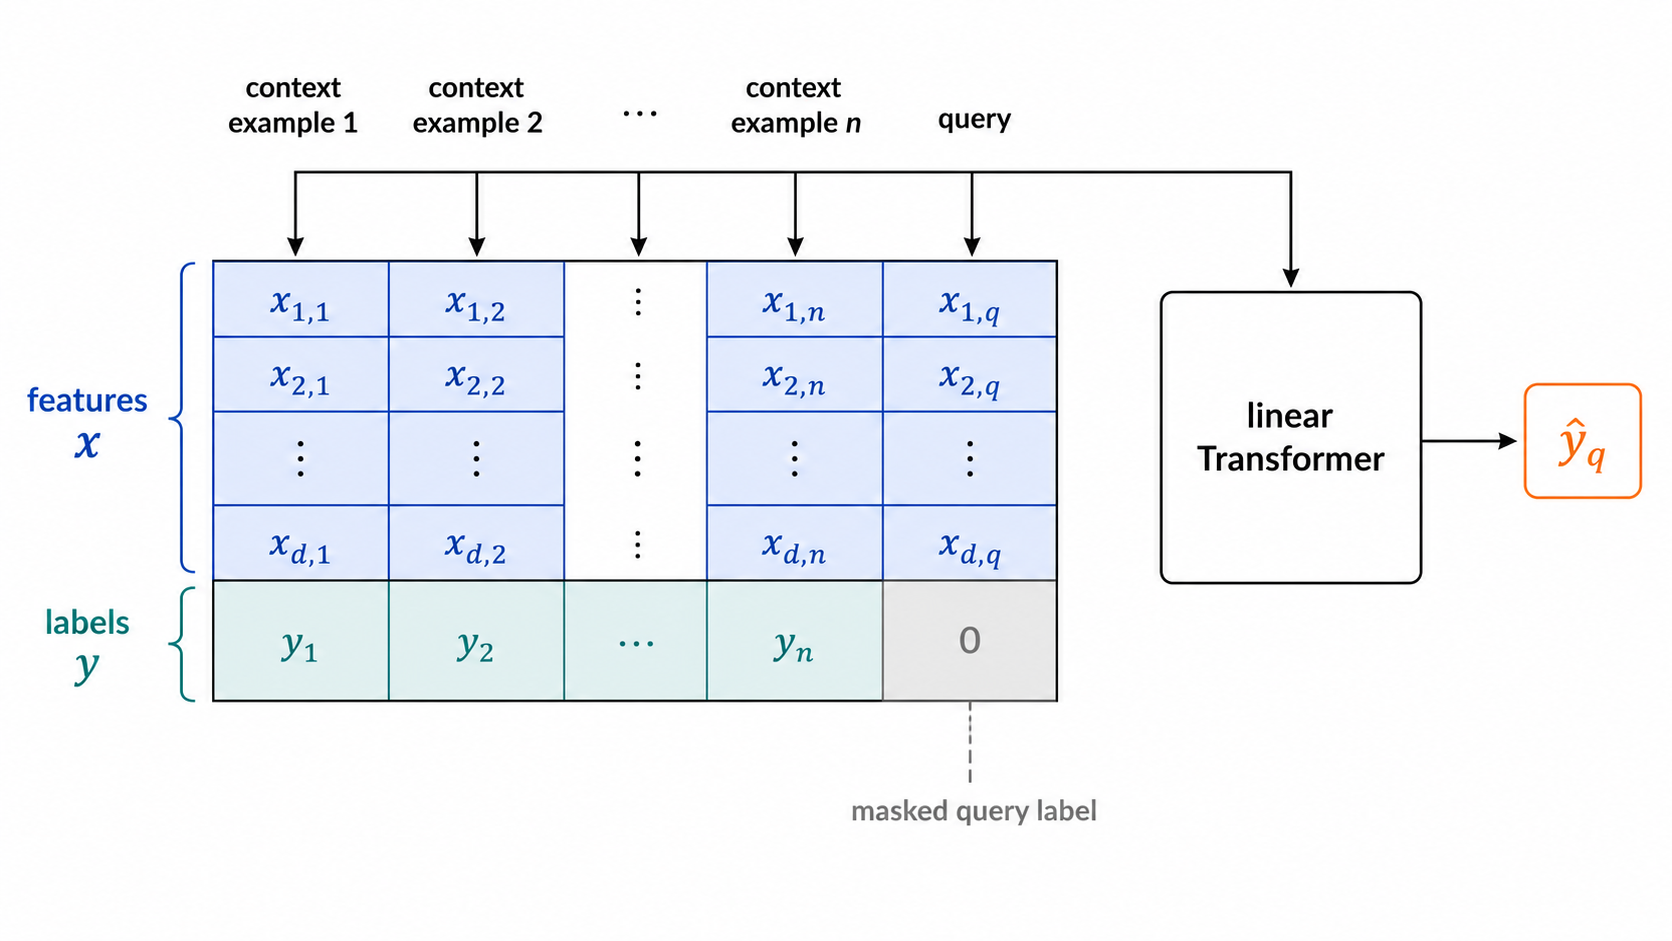
\includegraphics[width=\linewidth]{ai_linear_regression_structure.png}
  \caption{Conceptual structure of the linear-regression prompt. The query label is masked, so the model must infer the task from context examples.}
  \label{fig:ai_prompt}
\end{figure}

\subsection{Linear Self-Attention}
The paper removes softmax to obtain a tractable linear attention layer. Let
\begin{equation}
M =
\begin{bmatrix}
I_n & 0\\
0 & 0
\end{bmatrix}
\in \R^{(n+1)\times(n+1)}.
\end{equation}
The mask ensures that attention uses only the labeled context examples. For learnable matrices $P,Q \in \R^{(d+1)\times(d+1)}$, the attention map is
\begin{equation}
\operatorname{Attn}_{P,Q}(Z)=PZM(Z^\top QZ).
\end{equation}
An $L$-layer linear Transformer evolves by
\begin{equation}
Z_{\ell+1}=Z_\ell+\frac{1}{n}\operatorname{Attn}_{P_\ell,Q_\ell}(Z_\ell),
\quad \ell=0,\ldots,L-1.
\end{equation}
The prediction is defined as
\begin{equation}
\widehat{y} = -[Z_L]_{d+1,n+1}.
\end{equation}
The training objective is the expected squared ICL loss over random prompts.

\section{Theoretical Mechanism}
\subsection{Single-Layer Global Optimum}
The first major result characterizes the global optimum for a single attention layer. When $x^{(i)} \sim \N(0,\Sigma)$ and $\wstar \sim \N(0,I)$, the optimal $Q_0$ has a top-left block aligned with the inverse covariance eigenbasis. In the isotropic special case $\Sigma=I_d$, the solution reduces to a scaled identity direction. Figure \ref{fig:pse_theorem1} shows the formula from the PSE material.

\begin{figure}[!t]
  \centering
  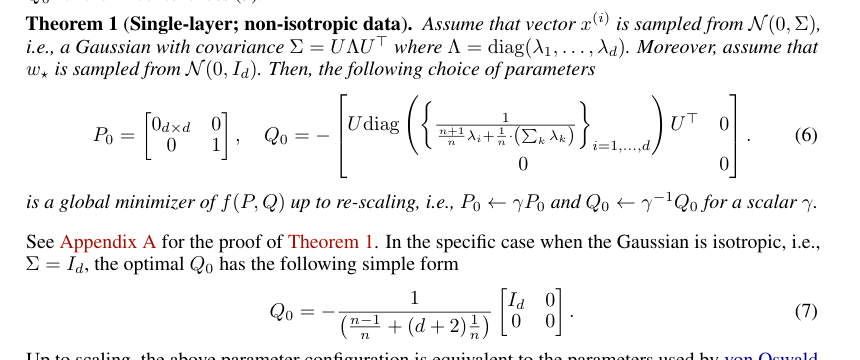
\includegraphics[width=0.95\linewidth]{pse_theorem1_formula.png}
  \caption{PSE formula for the single-layer global optimum. The learned matrix corresponds to one step of preconditioned gradient descent.}
  \label{fig:pse_theorem1}
\end{figure}

This optimum is algorithmic. The empirical risk of a linear predictor $w$ is
\begin{equation}
R_{\wstar}(w)=\frac{1}{2n}\sum_{i=1}^n (w^\top x^{(i)}-\wstar^\top x^{(i)})^2.
\end{equation}
Starting from $w_0=0$, one step of preconditioned gradient descent is
\begin{equation}
w_1=w_0-A\nabla R_{\wstar}(w_0)
=\frac{1}{n}A\sum_{i=1}^n y^{(i)}x^{(i)}.
\end{equation}
With the optimal attention parameters, the Transformer prediction equals $\langle w_1,x^{(n+1)}\rangle$ for an appropriate preconditioner $A$. Thus, the global optimum is not only an accurate predictor; it implements a classical optimization step. The finite-sample correction inside the preconditioner is also important. When the number of context examples is small, the coefficient is not simply $\Sigma^{-1}$. It contains a term depending on the trace of the covariance and on $n$. This is why the result has both optimization and statistical meaning: the model adapts to curvature and to uncertainty caused by limited context.

\subsection{Multi-Layer Sparse Parameterization}
The paper then studies a sparse parameterization
\begin{equation}
P_i =
\begin{bmatrix}
0_{d\times d} & 0\\
0 & 1
\end{bmatrix},
\quad
Q_i =
-
\begin{bmatrix}
A_i & 0\\
0 & 0
\end{bmatrix}.
\end{equation}
Under this constraint, the feature rows remain fixed and the label row is updated. The forward pass is equivalent to
\begin{equation}
w_{\ell+1}^{\mathrm{gd}} =
w_\ell^{\mathrm{gd}} - A_\ell \nabla R_{\wstar}(w_\ell^{\mathrm{gd}}),
\quad w_0^{\mathrm{gd}}=0.
\end{equation}
Therefore, depth corresponds to optimization iterations. For non-isotropic data with $x^{(i)}\sim\N(0,\Sigma)$ and $\wstar\sim\N(0,\Sigma^{-1})$, Theorem 3 states that parameters of the form $A_\ell=a_\ell\Sigma^{-1}$ essentially contain critical points of the ICL loss. This is a distribution-level preconditioner: for large $n$, the Hessian $XX^\top/n$ concentrates near $\Sigma$, so $\Sigma^{-1}$ improves conditioning.

\subsection{Relaxed Parameterization and Feature Transformation}
Theorem 4 removes part of the sparsity restriction by allowing
\begin{equation}
P_i =
\begin{bmatrix}
B_i & 0\\
0 & 1
\end{bmatrix},
\quad
Q_i =
\begin{bmatrix}
A_i & 0\\
0 & 0
\end{bmatrix}.
\end{equation}
The resulting critical-point structure satisfies $A_i=a_i\Sigma^{-1}$ and $B_i=b_iI$. This is more than standard preconditioned gradient descent. The $A_i$ matrices precondition label-driven gradient steps, while the $B_i$ matrices transform feature rows, approximately improving the conditioning of the Gram matrix. This connects the learned Transformer to the GD++ mechanism discussed by von Oswald et al. \cite{von2023transformers}.

\subsection{Why the Mechanism Is Nontrivial}
The theoretical mechanism is nontrivial because the model never receives the command ``run gradient descent.'' It only receives prediction loss over random prompts. If the trained parameter structure matches preconditioned GD, this means the training distribution and architecture induce an optimization algorithm implicitly. The results therefore support an algorithmic view of ICL: a Transformer layer can be treated as a computational step, and the learned weights define how that step adapts to the data distribution.

This does not mean that every Transformer layer in a large language model literally performs the same update. The claim is narrower and more rigorous: in a controlled linear-regression setting, the loss landscape contains optima or near-critical structures with a clear preconditioned-gradient interpretation. That is exactly the kind of statement that can be reproduced and evaluated with structural metrics.

\begin{figure}[!t]
  \centering
  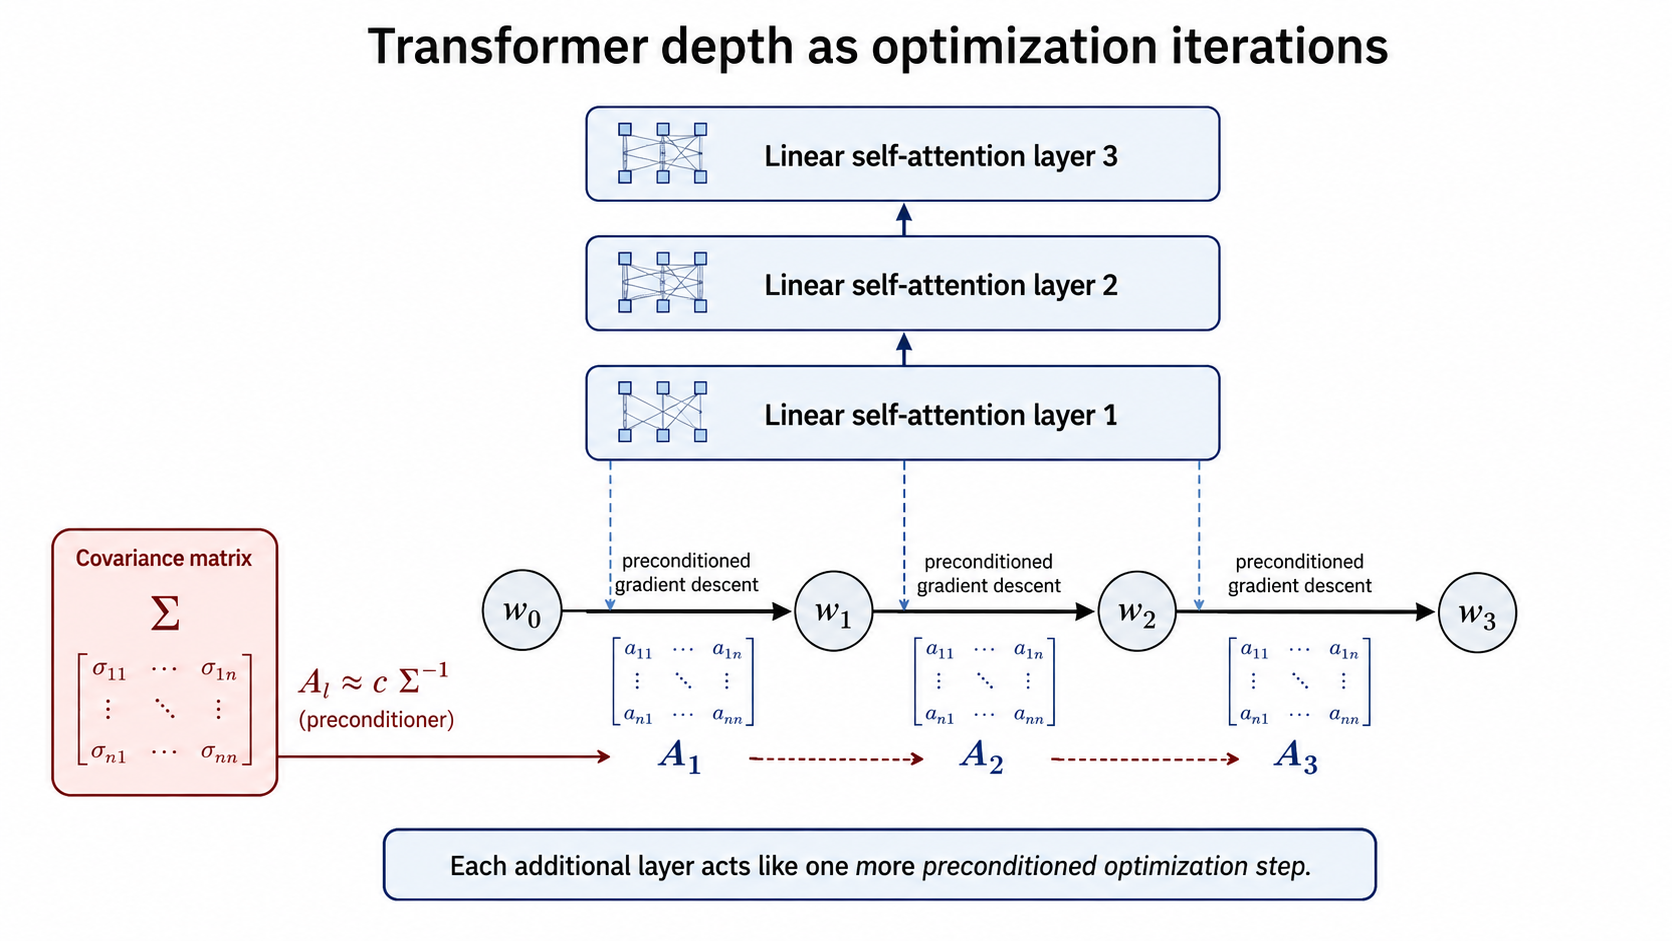
\includegraphics[width=\linewidth]{ai_theoretical_mechanism.png}
  \caption{Conceptual view of the paper's mechanism: Transformer layers act as learned optimization iterations, and the learned matrices define the preconditioning geometry.}
  \label{fig:ai_mechanism}
\end{figure}

\subsection{Loss-Landscape Interpretation}
The most theoretical part of the target paper is not the forward equivalence alone. The stronger statement is about the loss landscape of training over random prompts. Under the sparse parameterization, the model class can be viewed as a search space over $L$-step gradient-based algorithms. The loss $f(A)$ is the expected query prediction error after applying those $L$ learned steps. Theorem 3 identifies a structured subset
\begin{equation}
\mathcal{S}_A=\{A: A_\ell=a_\ell\Sigma^{-1},\ \ell=0,\ldots,L-1\}
\end{equation}
whose points can have arbitrarily small gradient norm. This is weaker than saying every training run must converge to that set, but stronger than saying such weights merely exist by construction. It links the stationary structure of the training objective to a classical optimizer.

Theorem 4 performs the same type of reasoning after enlarging the parameter space. The relevant structured subset becomes
\begin{equation}
\mathcal{S}_{A,B}=\{(A,B):A_\ell=a_\ell\Sigma^{-1},\ B_\ell=b_\ell I\}.
\end{equation}
This subset has a two-part interpretation. The $A_\ell$ matrices determine how label residuals update the implicit predictor, while the $B_\ell$ matrices reshape the feature representation. A useful way to read the theorem is that training can discover a coordinate system in which the regression problem is easier to optimize.

\subsection{Statistical Meaning of the Preconditioner}
The preconditioner is not an arbitrary acceleration device. In the Gaussian linear-regression setting, $\Sigma$ is the population covariance of the input features. The empirical Hessian of the squared loss is proportional to $XX^\top/n$. When $n$ is large, this matrix concentrates around $\Sigma$, so $\Sigma^{-1}$ approximates a population-level Newton direction. When $n$ is small, however, the empirical Hessian is noisy and may be poorly conditioned. The single-layer theorem captures this by including a finite-sample correction term in the optimal coefficient. This is why the paper also has a sample-complexity flavor: the same preconditioner must balance curvature adaptation and uncertainty from limited in-context examples.

This interpretation also explains why the report emphasizes structural metrics rather than only final prediction loss. If $A_i$ simply became close to $I$, the learned procedure would resemble ordinary GD. If $\Sigma^{1/2}A_i\Sigma^{1/2}$ becomes close to a scaled identity, then $A_i$ is close to $\Sigma^{-1}$ in the appropriate basis. The latter is the theoretical signature of preconditioned GD.

\section{Derivation Sketch and Reproduction Criteria}
\subsection{From Attention Update to Gradient Step}
It is helpful to spell out why the sparse attention layer becomes a gradient step. Let $X=[x^{(1)},\ldots,x^{(n)}]$ be the context feature matrix, and let $y=[y^{(1)},\ldots,y^{(n)}]^\top$. Suppose the label row of $Z_\ell$ encodes current prediction residuals for the context and query. Under the sparse parameterization, the feature rows do not change, and the only relevant learned matrix is $A_\ell$ inside $Q_\ell$. The masked attention term uses the context columns through $M$, so the query update depends on inner products between the query feature and the context features. Algebraically, this creates a term proportional to
\begin{equation}
x^{(n+1)\top}A_\ell X\left(X^\top w_\ell-y\right).
\end{equation}
Up to the paper's sign convention and the factor $1/n$, this is exactly the query prediction change produced by
\begin{equation}
w_{\ell+1}=w_\ell-A_\ell\frac{1}{n}X(X^\top w_\ell-y).
\end{equation}
The vector on the right is $\nabla R_{\wstar}(w_\ell)$. Thus, the attention layer does not merely resemble gradient descent metaphorically; in this restricted parameter regime, its forward computation is the same algebraic object as a preconditioned gradient step.

\subsection{Role of Masking and the Query Zero Label}
Two implementation details are essential for the theory. The mask prevents the query column from being used as a labeled training example. The zero query label keeps the prompt format rectangular while avoiding leakage of $\wstar^\top x^{(n+1)}$. If either detail is changed, the model no longer corresponds to the same ICL objective. In a reproduction project, these details are therefore not engineering trivia; they are part of the mathematical object being tested.

The sign convention is also important. The prediction is $-[Z_L]_{d+1,n+1}$, so the label-row state is interpreted with a negative sign. A mismatch in this sign would make the apparent update direction disagree with the gradient-descent interpretation even if the rest of the architecture were correct.

\subsection{What CRE Can and Cannot Verify}
The CRE experiments are designed as structural checks. They can verify whether the observed trained parameters move in the direction predicted by the theorems. They cannot prove the theorem again, and they cannot rule out other parameter regions of the non-convex landscape. This distinction is important for a rigorous course report: reproduction evidence supports the paper's claims by matching predicted observables, but the mathematical guarantee still comes from the original analysis.

\begin{table}[!t]
\centering
\caption{Structural reproduction criteria used in CRE.}
\label{tab:criteria}
\begin{tabular}{p{0.20\linewidth}p{0.33\linewidth}p{0.35\linewidth}}
\toprule
Claim & Expected evidence & Possible contradiction\\
\midrule
Theorem 3 & Rotated $A_i$ distances decrease more than raw distances & Raw $A_i$ becomes identity-like with no covariance-adjusted advantage\\
Theorem 4 & Both $B_i$ and rotated $A_i$ distances decrease & Only prediction loss drops while matrices remain unstructured\\
Context length & More examples generally reduce test loss & Loss does not improve with additional context\\
\bottomrule
\end{tabular}
\end{table}

\subsection{Why the Result Concerns Computational Complexity}
The model has a fixed number of layers, so it has a fixed number of optimization steps. This is a computational constraint. Ordinary gradient descent may require many iterations on an ill-conditioned problem, while preconditioning can reduce the number of effective iterations. The paper's result therefore says that the trained Transformer can use its limited depth more efficiently by learning a covariance-aware update. In course terminology, this is why the paper is best categorized under optimization error and computational complexity rather than only expressivity.

\section{Experimental Design}
\subsection{Official Evidence and Reproduction Evidence}
Table \ref{tab:theory_summary} summarizes the main theoretical results relevant to the course report. Figure \ref{fig:pse_summary} shows the PSE table from the paper analysis assets.

\begin{table}[!t]
\centering
\caption{Main theoretical results and their algorithmic interpretation.}
\label{tab:theory_summary}
\begin{tabular}{p{0.14\linewidth}p{0.30\linewidth}p{0.40\linewidth}}
\toprule
Result & Model setting & Interpretation\\
\midrule
Theorem 1 & One linear attention layer & Global optimum implements one preconditioned GD step\\
Theorem 3 & Multi-layer sparse parameters & Critical structure implements $\Sigma^{-1}$-preconditioned GD\\
Theorem 4 & Relaxed $A_i,B_i$ parameters & Preconditioned steps plus feature transformation\\
\bottomrule
\end{tabular}
\end{table}

\begin{figure}[!t]
  \centering
  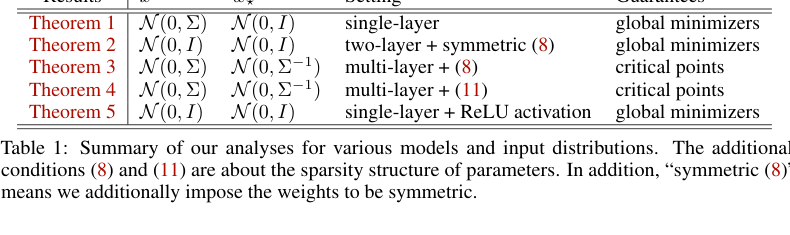
\includegraphics[width=\linewidth]{pse_table1_summary.png}
  \caption{PSE summary of theoretical regimes in the NeurIPS 2023 paper.}
  \label{fig:pse_summary}
\end{figure}

Our CRE experiments focus on three checks. First, the constrained Theorem 3 setting should show that rotated matrices $\Sigma^{1/2}A_i\Sigma^{1/2}$ move closer to a scaled identity than raw $A_i$. Second, the relaxed Theorem 4 setting should show both $A_i$ and $B_i$ approaching the predicted structures. Third, a context-length extension should show how additional in-context examples reduce test loss, connecting the main optimization story to a sample-complexity perspective.

\begin{table}[!t]
\centering
\caption{CRE experiment settings used for the report evidence.}
\label{tab:cre_setup}
\begin{tabular}{p{0.31\linewidth}p{0.55\linewidth}}
\toprule
Experiment & Course-scale setting\\
\midrule
Theorem 3 & Three-layer linear Transformer, constrained sparse parameters, $d=5$, $n=20$, two random seeds\\
Theorem 4 & Three-layer relaxed linear Transformer with learned $A_i$ and $B_i$, $d=5$, $n=20$, two random seeds\\
Context length & $N\in\{4,8,12,16,20\}$, comparing Transformer, GD, PGD, and OLS\\
\bottomrule
\end{tabular}
\end{table}

\subsection{Metrics}
The structural metric is
\begin{equation}
\Dist(M,I)=\min_\alpha \frac{\|M-\alpha I\|_F}{\|M\|_F}.
\end{equation}
For Theorem 3, the key comparison is $\Dist(\Sigma^{1/2}A_i\Sigma^{1/2},I)$ versus $\Dist(A_i,I)$. A successful structural reproduction should reduce the former more strongly than the latter. For Theorem 4, the same rotated $A_i$ metric is paired with $\Dist(B_i,I)$.

\section{PSE vs. CRE Results}
\subsection{Theorem 3: Constrained Preconditioned GD}
The PSE result in Figure \ref{fig:pse_t3} shows loss reduction and decreasing rotated distances for the constrained setting. The conceptual point is that the learned matrix is close to $\Sigma^{-1}$ in the covariance-adjusted basis, not close to ordinary identity-gradient descent in the raw basis.

\begin{figure}[!t]
  \centering
  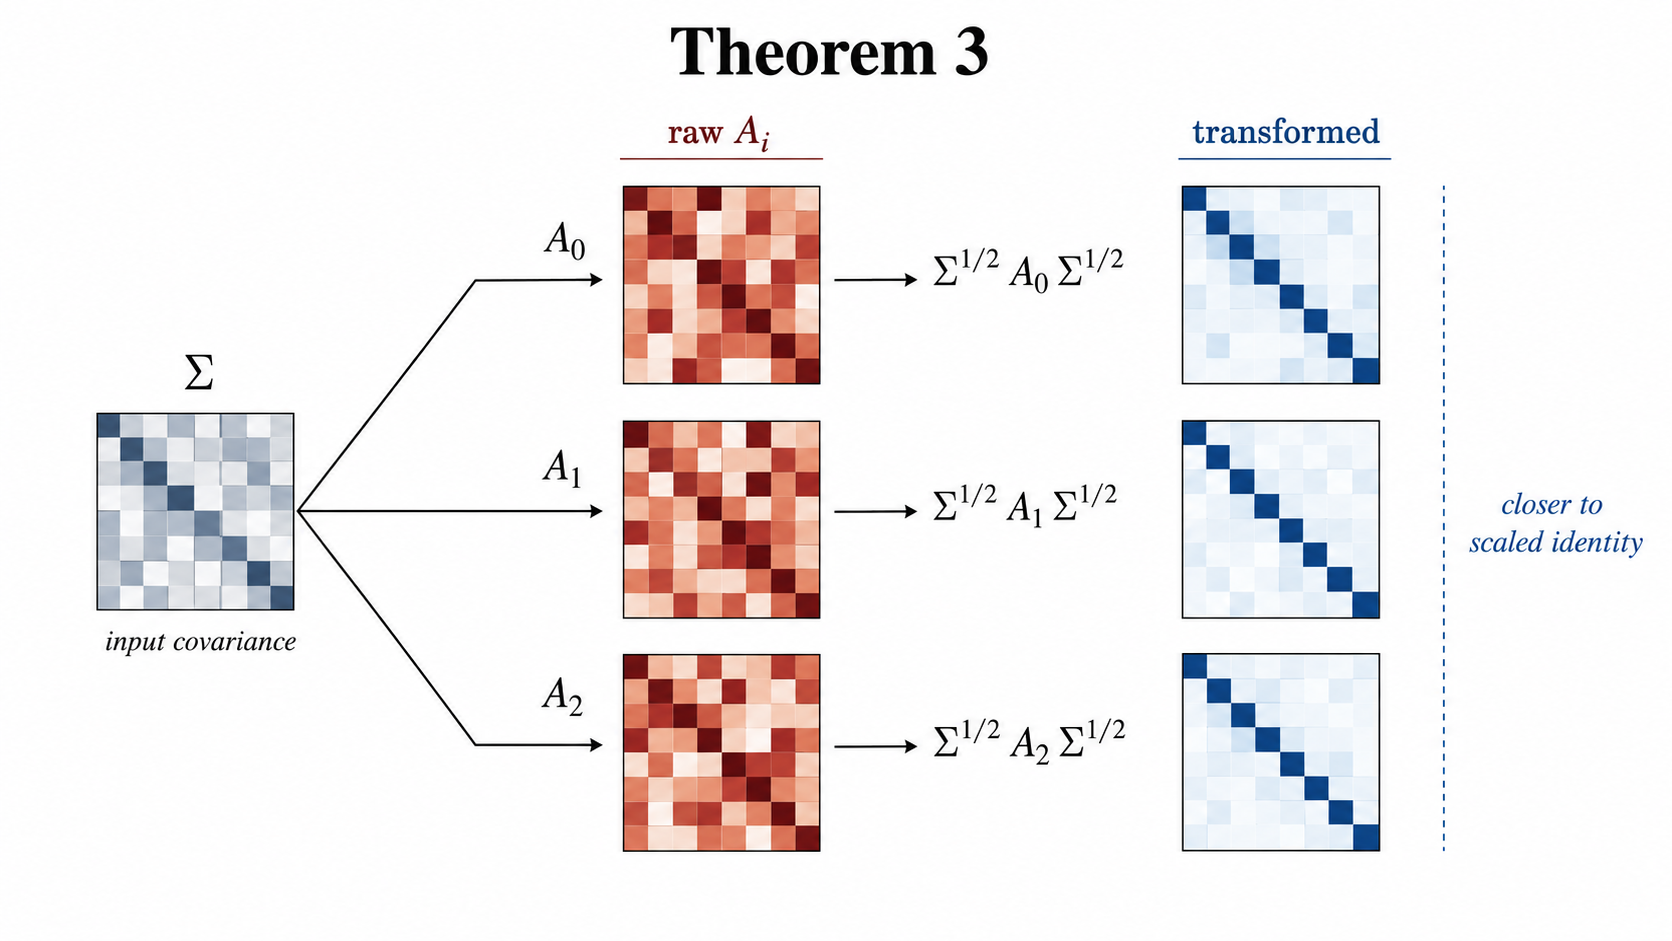
\includegraphics[width=\linewidth]{ai_theorem3_mechanism.png}
  \caption{Conceptual Theorem 3 mechanism. The sparse setting tests whether the learned $A_i$ matrices align with $\Sigma^{-1}$ after covariance rotation.}
  \label{fig:ai_t3}
\end{figure}

\begin{figure}[!t]
  \centering
  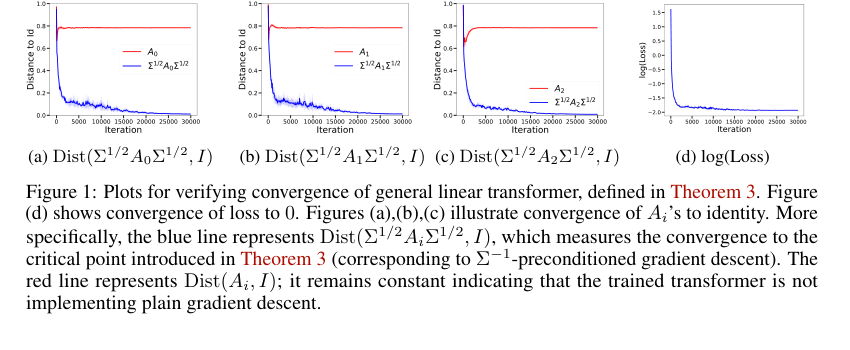
\includegraphics[width=\linewidth]{pse_theorem3_curves.png}
  \caption{PSE Theorem 3 curves. The rotated distance decreases, supporting the $\Sigma^{-1}$ preconditioner interpretation.}
  \label{fig:pse_t3}
\end{figure}

The CRE counterpart follows the same structural logic. The log loss decreases from $1.641430$ to $-1.580373$. For $A_0$, the rotated distance decreases from $0.950218$ to $0.169304$, while the raw distance decreases only from $0.999481$ to $0.769688$. Similar patterns appear for $A_1$ and $A_2$. This supports the same theoretical interpretation: the trained model is better described by a covariance-aware preconditioner than by plain gradient descent.

The contrast between raw and rotated distances is essential. In a non-isotropic distribution, the identity matrix is not the theoretically preferred direction. A method that ignores covariance must use small conservative steps along high-variance directions and therefore wastes computation along low-variance directions. A preconditioned method rescales the geometry, so one layer can behave like a more effective optimization step. The CRE result therefore validates the relevant theoretical invariant: after rotating by $\Sigma^{1/2}$, the learned matrices become identity-like even when the raw matrices do not.

\begin{table}[!t]
\centering
\caption{CRE Theorem 3 structural metrics. Lower distance means closer to a scaled identity.}
\label{tab:t3_metrics}
\begin{tabular}{lrrr}
\toprule
Metric & First & Final & Change\\
\midrule
Log loss & 1.6414 & -1.5804 & -3.2218\\
Rotated $A_0$ distance & 0.9502 & 0.1693 & -0.7809\\
Raw $A_0$ distance & 0.9995 & 0.7697 & -0.2298\\
Rotated $A_1$ distance & 0.9757 & 0.3928 & -0.5830\\
Raw $A_1$ distance & 0.9841 & 0.8120 & -0.1721\\
Rotated $A_2$ distance & 0.9654 & 0.2126 & -0.7528\\
Raw $A_2$ distance & 0.9548 & 0.7573 & -0.1976\\
\bottomrule
\end{tabular}
\end{table}

\begin{figure}[!t]
\centering
\begin{subfigure}{0.48\linewidth}
  \centering
  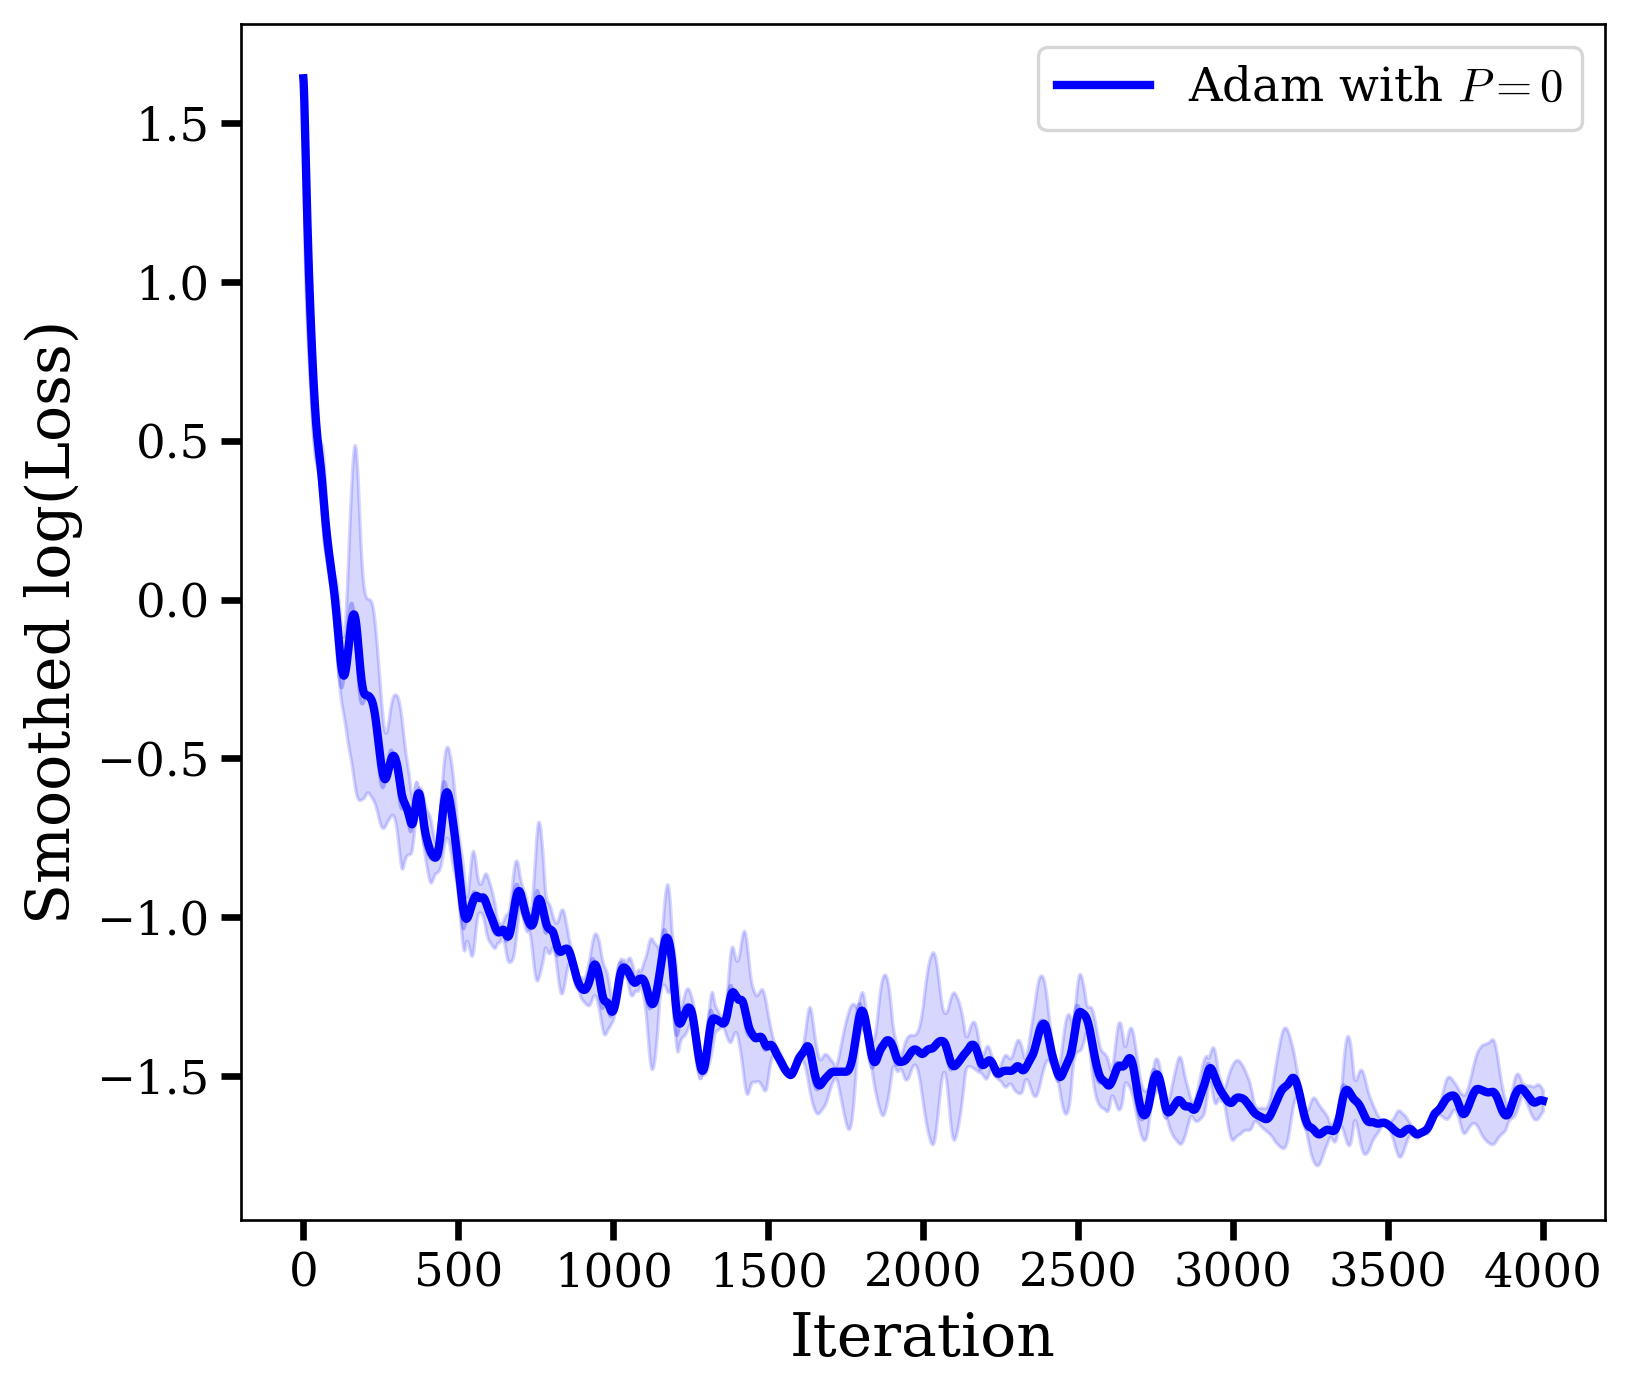
\includegraphics[width=\linewidth]{cre_t3_loss_smooth.png}
  \caption{CRE loss}
\end{subfigure}
\hfill
\begin{subfigure}{0.48\linewidth}
  \centering
  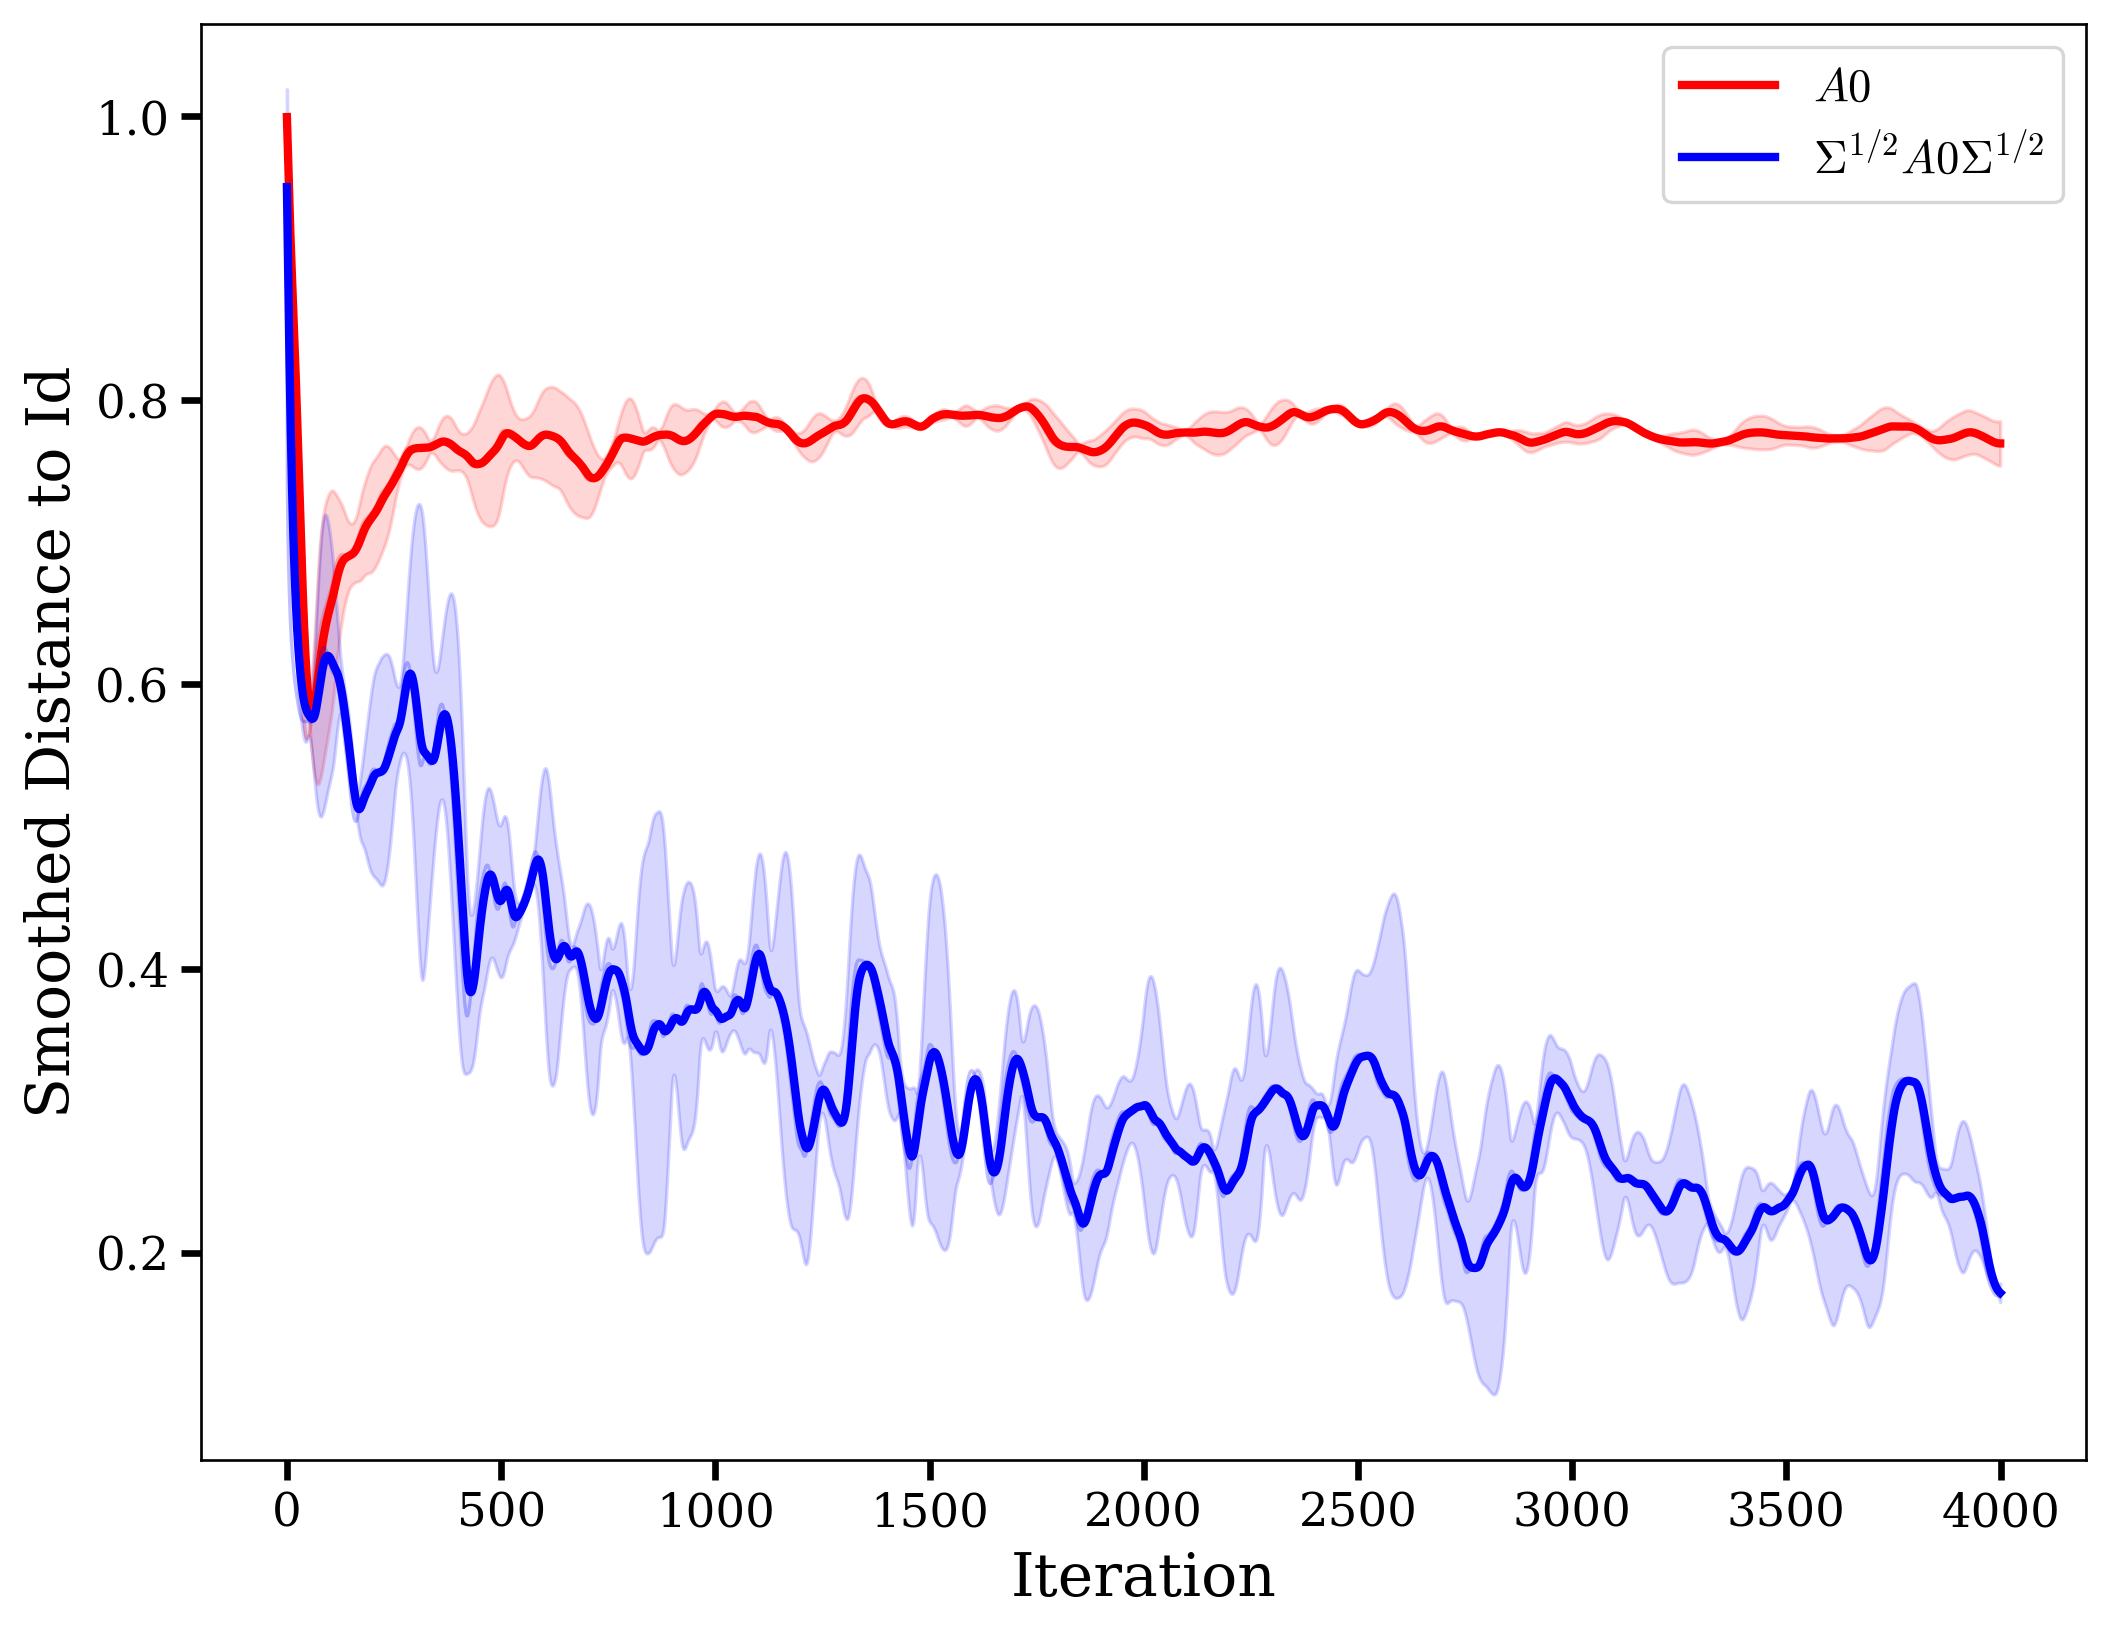
\includegraphics[width=\linewidth]{cre_t3_a0_distance_smooth.png}
  \caption{CRE $A_0$ distance}
\end{subfigure}
\caption{CRE Theorem 3 evidence. The course-scale run preserves the key qualitative pattern: loss falls and the rotated matrix becomes much closer to a scaled identity.}
\label{fig:cre_t3}
\end{figure}

\begin{figure}[!t]
  \centering
  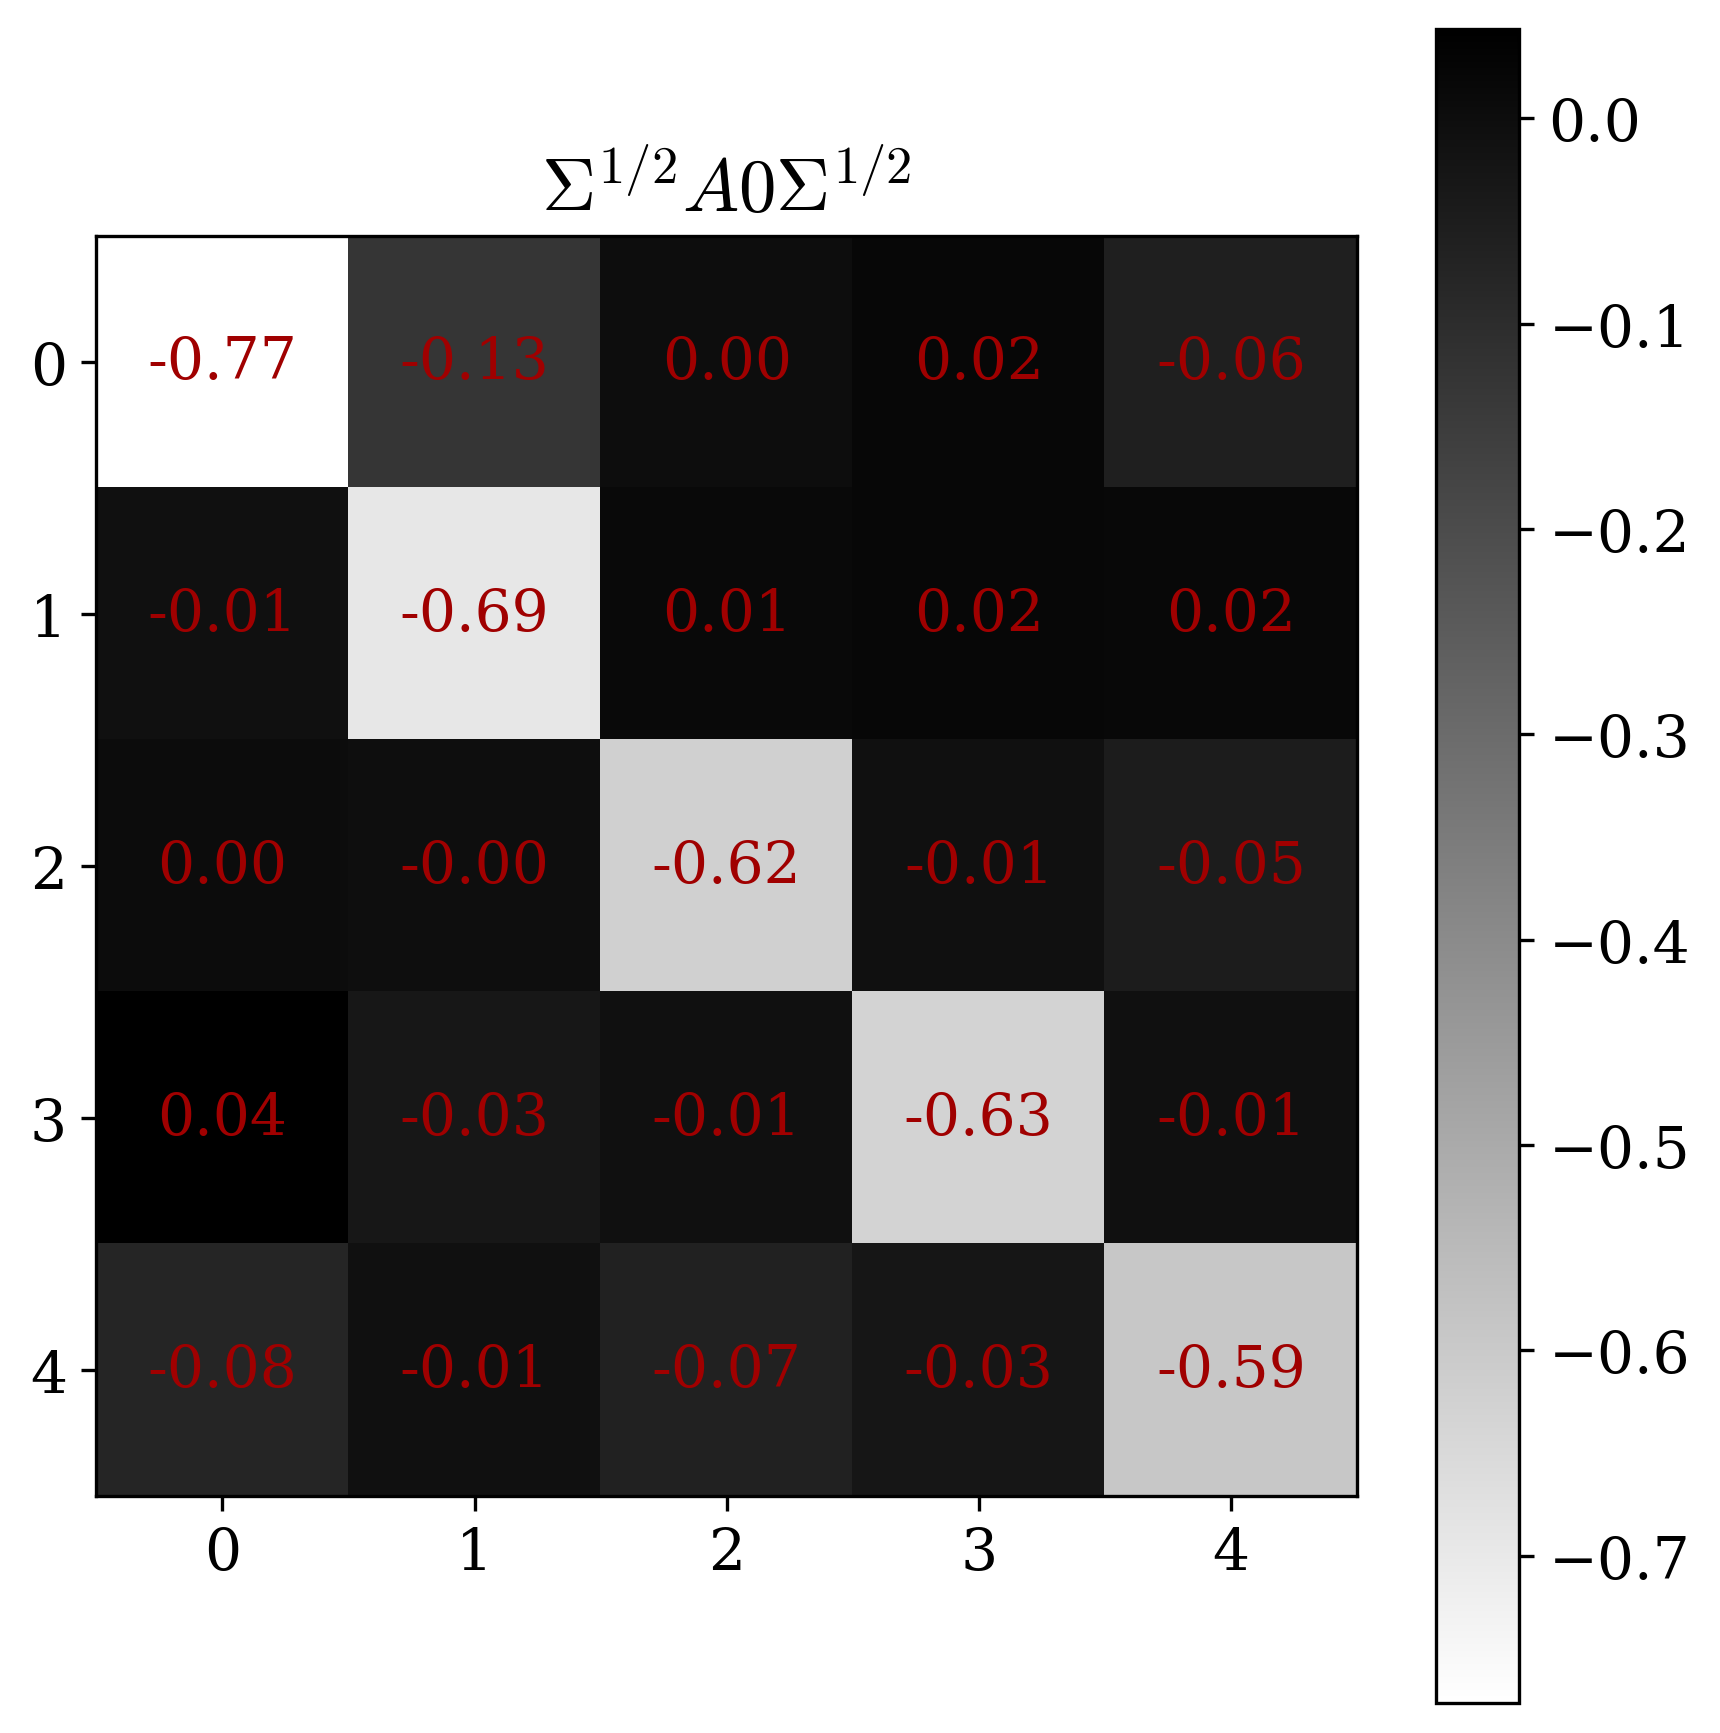
\includegraphics[width=0.72\linewidth]{cre_t3_a0_heatmap.png}
  \caption{CRE final heatmap for the rotated $A_0$ structure in the constrained setting.}
  \label{fig:cre_t3_heatmap}
\end{figure}

\begin{figure}[!t]
  \centering
  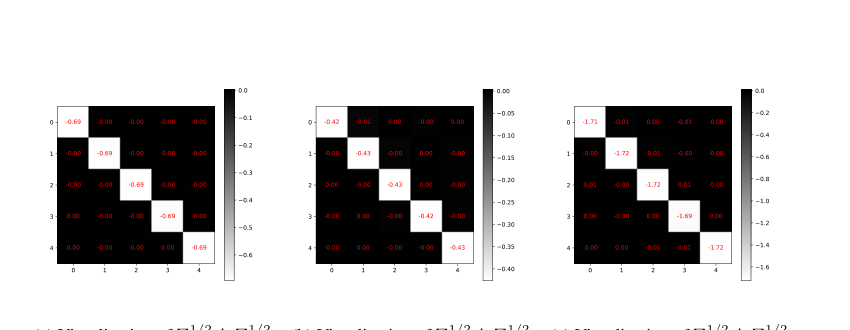
\includegraphics[width=\linewidth]{pse_theorem3_heatmaps.png}
  \caption{PSE Theorem 3 final heatmaps. These heatmaps motivate the CRE heatmap check.}
  \label{fig:pse_t3_heatmap}
\end{figure}

\subsection{Theorem 4: Relaxed Feature Transformation}
Theorem 4 predicts that, under relaxed parameters, the model can learn both preconditioned gradient steps and feature transformations. The PSE evidence in Figure \ref{fig:pse_t4} shows decreasing distances for $B_i$ and rotated $A_i$, and the PSE heatmaps in Figure \ref{fig:pse_t4_heatmap} show that $B_0,B_1$ are close to scaled identity matrices.

\begin{figure}[!t]
  \centering
  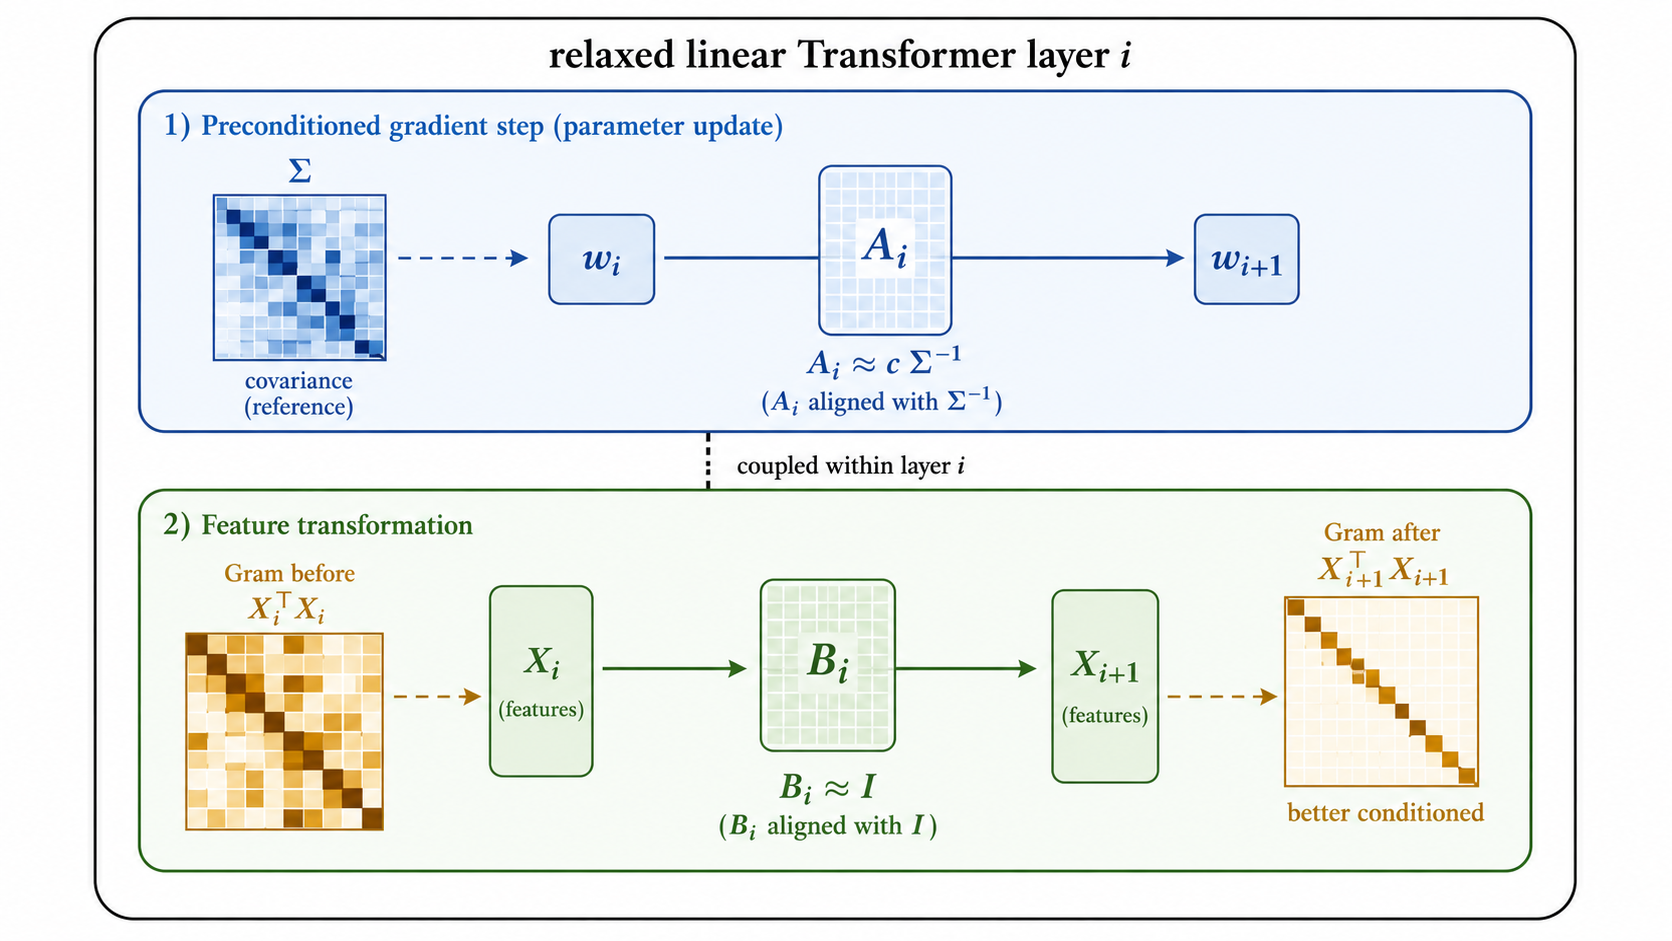
\includegraphics[width=\linewidth]{ai_theorem4_feature_transformation.png}
  \caption{Conceptual Theorem 4 mechanism. The relaxed model combines preconditioned updates through $A_i$ with feature transformation through $B_i$.}
  \label{fig:ai_t4}
\end{figure}

\begin{figure}[!t]
  \centering
  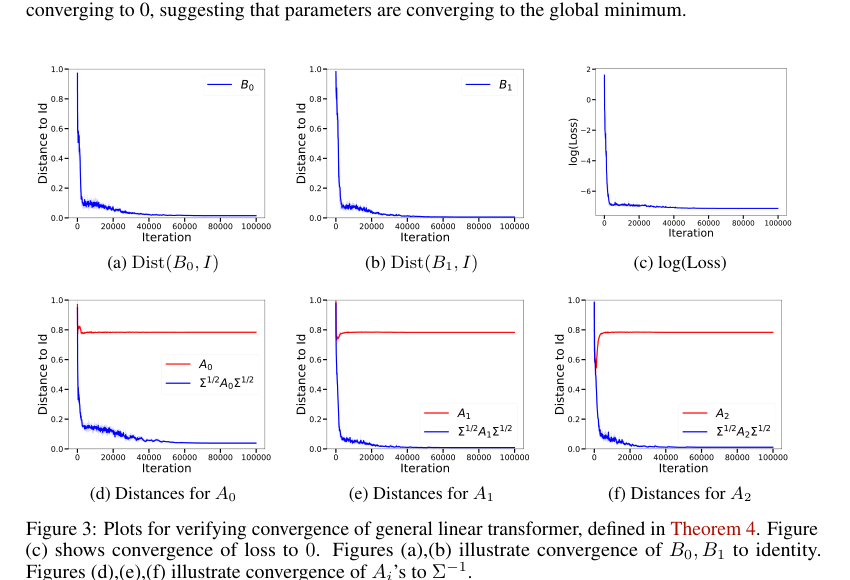
\includegraphics[width=\linewidth]{pse_theorem4_curves.png}
  \caption{PSE Theorem 4 curves for the relaxed setting.}
  \label{fig:pse_t4}
\end{figure}

\begin{figure}[!t]
  \centering
  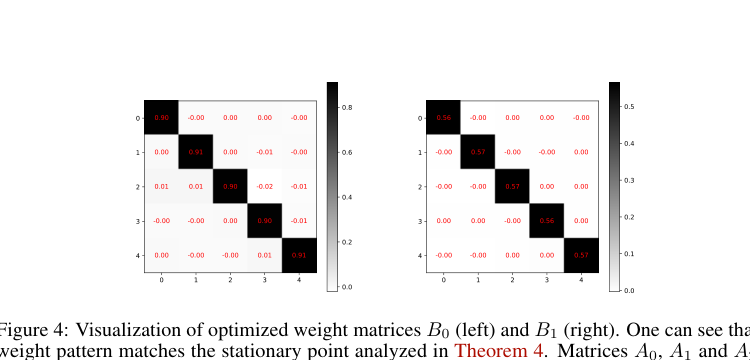
\includegraphics[width=\linewidth]{pse_theorem4_b_heatmaps.png}
  \caption{PSE Theorem 4 heatmaps for learned $B_i$ matrices.}
  \label{fig:pse_t4_heatmap}
\end{figure}

The CRE run also shows the expected qualitative movement. The log loss decreases from $1.641430$ to $-4.221714$. The final distances are lower for both feature-transform and preconditioning components: $B_0$ decreases from $0.997822$ to $0.558772$, $B_1$ from $0.966573$ to $0.477783$, $A_0$ from $0.950218$ to $0.373056$, $A_1$ from $0.975746$ to $0.376785$, and $A_2$ from $0.965415$ to $0.394170$. The course-scale curves do not claim exact paper-scale convergence, but they reproduce the central structural direction.

The relaxed setting is theoretically richer than the constrained setting because the model is no longer forced to keep the feature rows fixed. From an optimization viewpoint, this means the network is learning both an update rule and a representation transformation. The representation transformation can improve the condition number of the Gram matrix encountered by later layers. In this sense, the learned procedure is closer to a learned optimizer with an internal state transformation than to a fixed hand-written gradient method.

\begin{table}[!t]
\centering
\caption{CRE Theorem 4 structural metrics.}
\label{tab:t4_metrics}
\begin{tabular}{lrrr}
\toprule
Metric & First & Final & Change\\
\midrule
Log loss & 1.6414 & -4.2217 & -5.8631\\
$B_0$ distance & 0.9978 & 0.5588 & -0.4391\\
$B_1$ distance & 0.9666 & 0.4778 & -0.4888\\
$A_0$ distance & 0.9502 & 0.3731 & -0.5772\\
$A_1$ distance & 0.9757 & 0.3768 & -0.5990\\
$A_2$ distance & 0.9654 & 0.3942 & -0.5712\\
\bottomrule
\end{tabular}
\end{table}

\begin{figure}[!t]
\centering
\begin{subfigure}{0.48\linewidth}
  \centering
  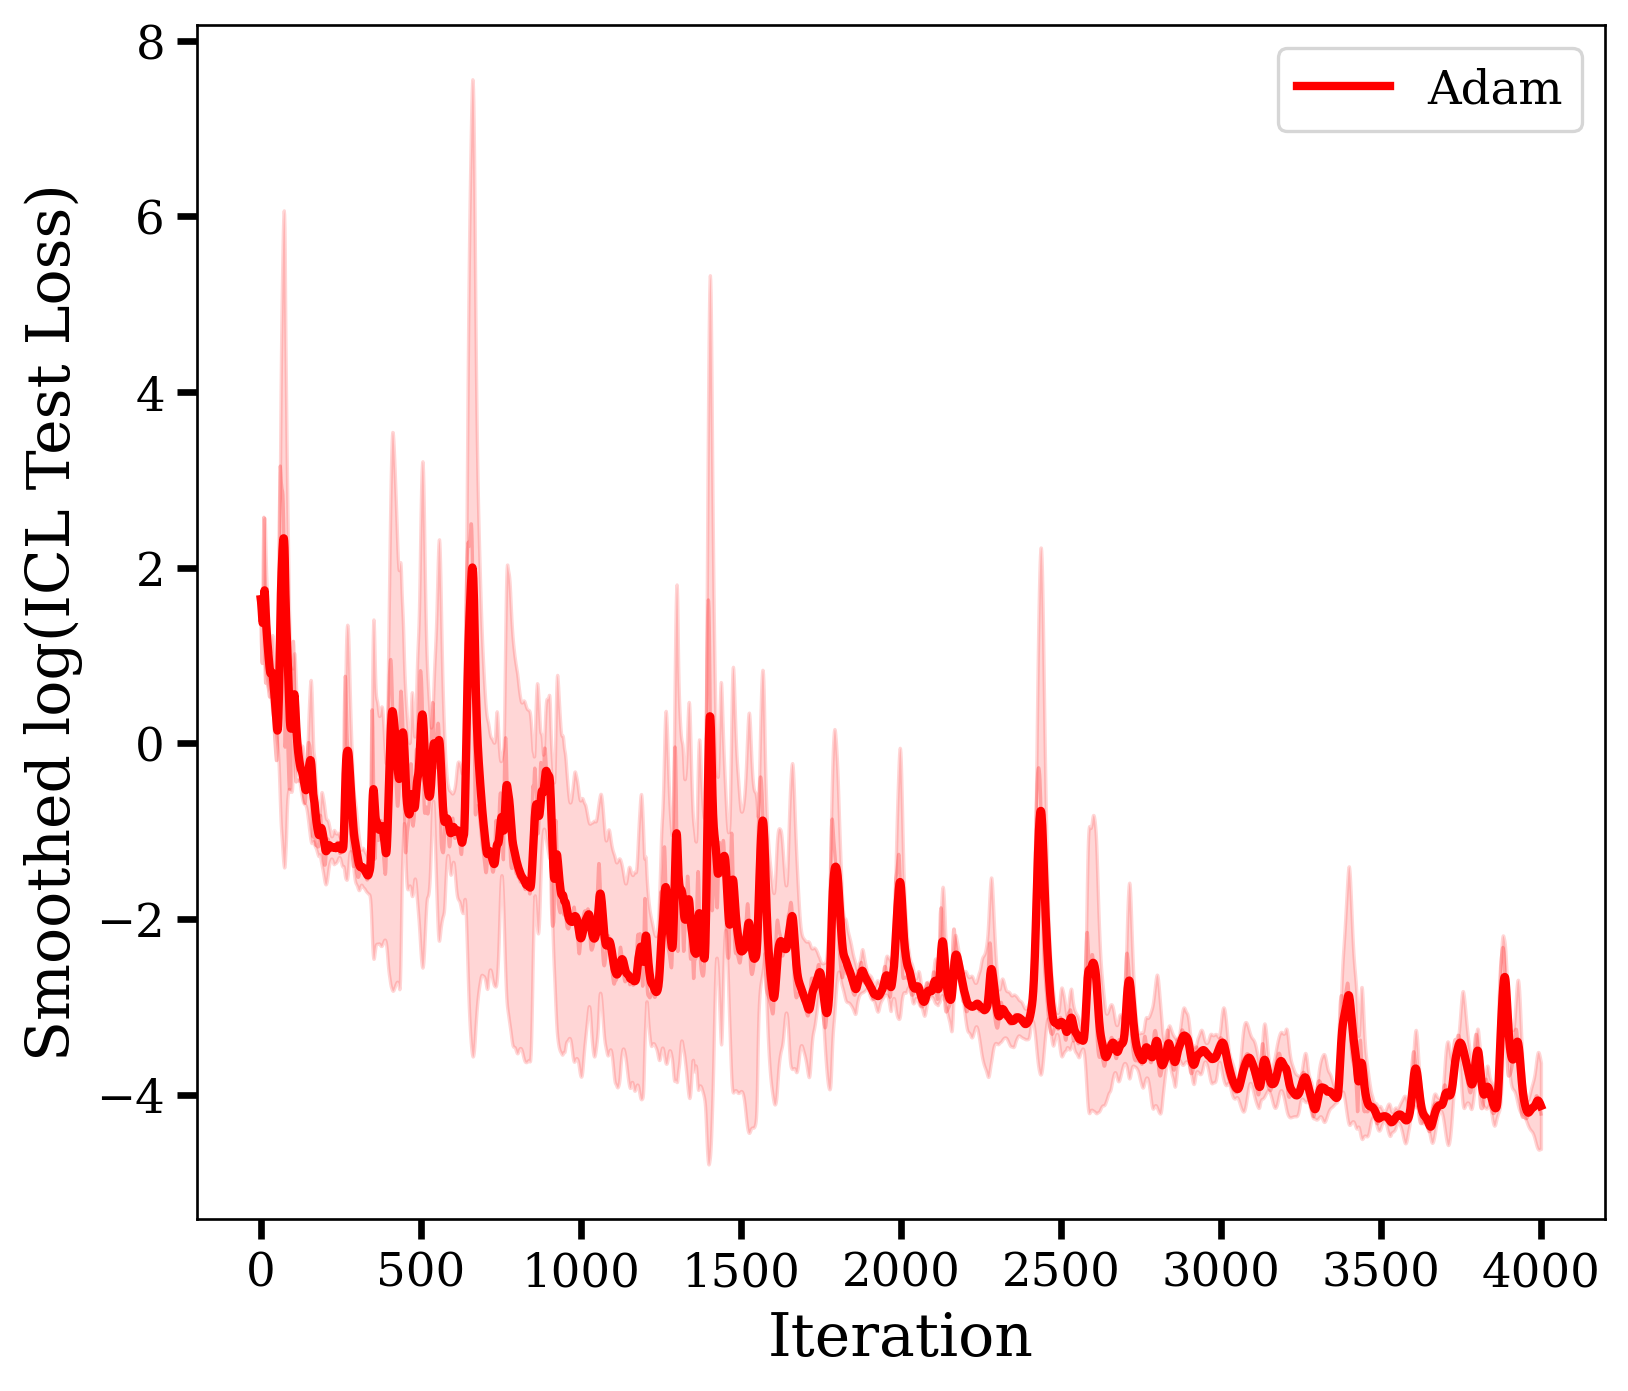
\includegraphics[width=\linewidth]{cre_t4_loss_smooth.png}
  \caption{CRE loss}
\end{subfigure}
\hfill
\begin{subfigure}{0.48\linewidth}
  \centering
  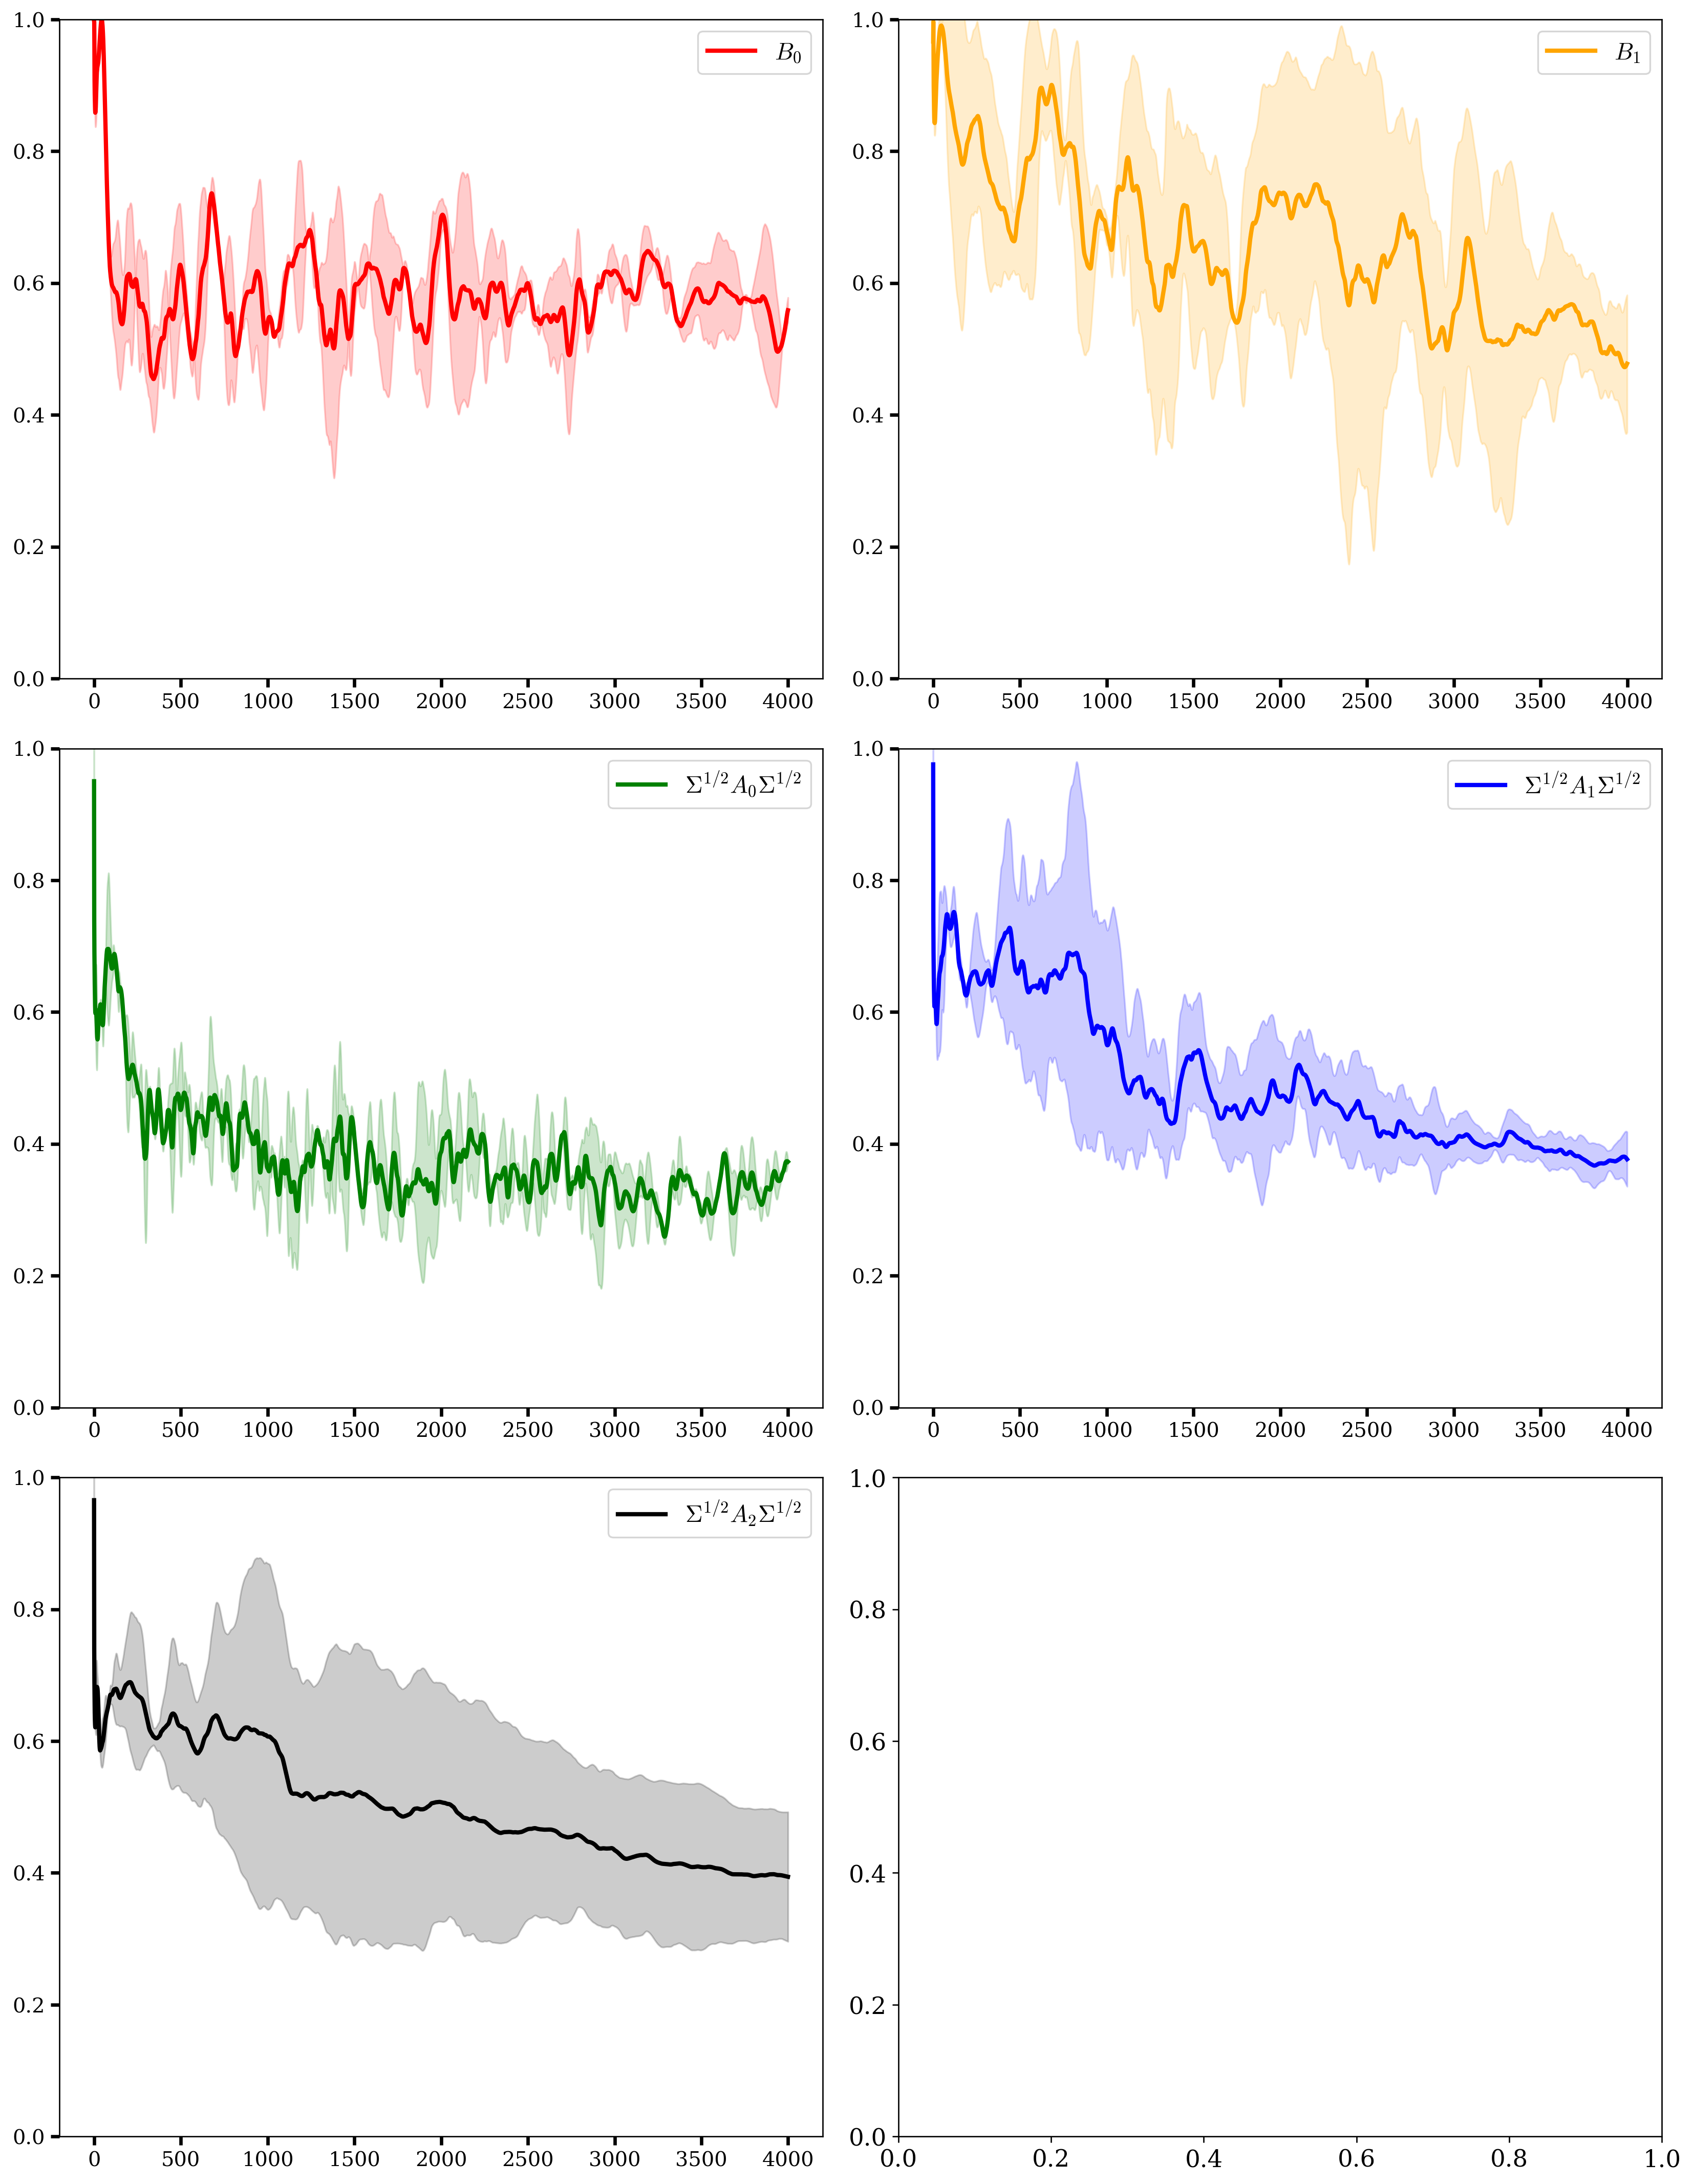
\includegraphics[width=\linewidth]{cre_t4_distance_panel.png}
  \caption{CRE distance panel}
\end{subfigure}
\caption{CRE Theorem 4 evidence. Both loss and structural distances move in the direction predicted by the relaxed critical-point theory.}
\label{fig:cre_t4}
\end{figure}

\begin{figure}[!t]
  \centering
  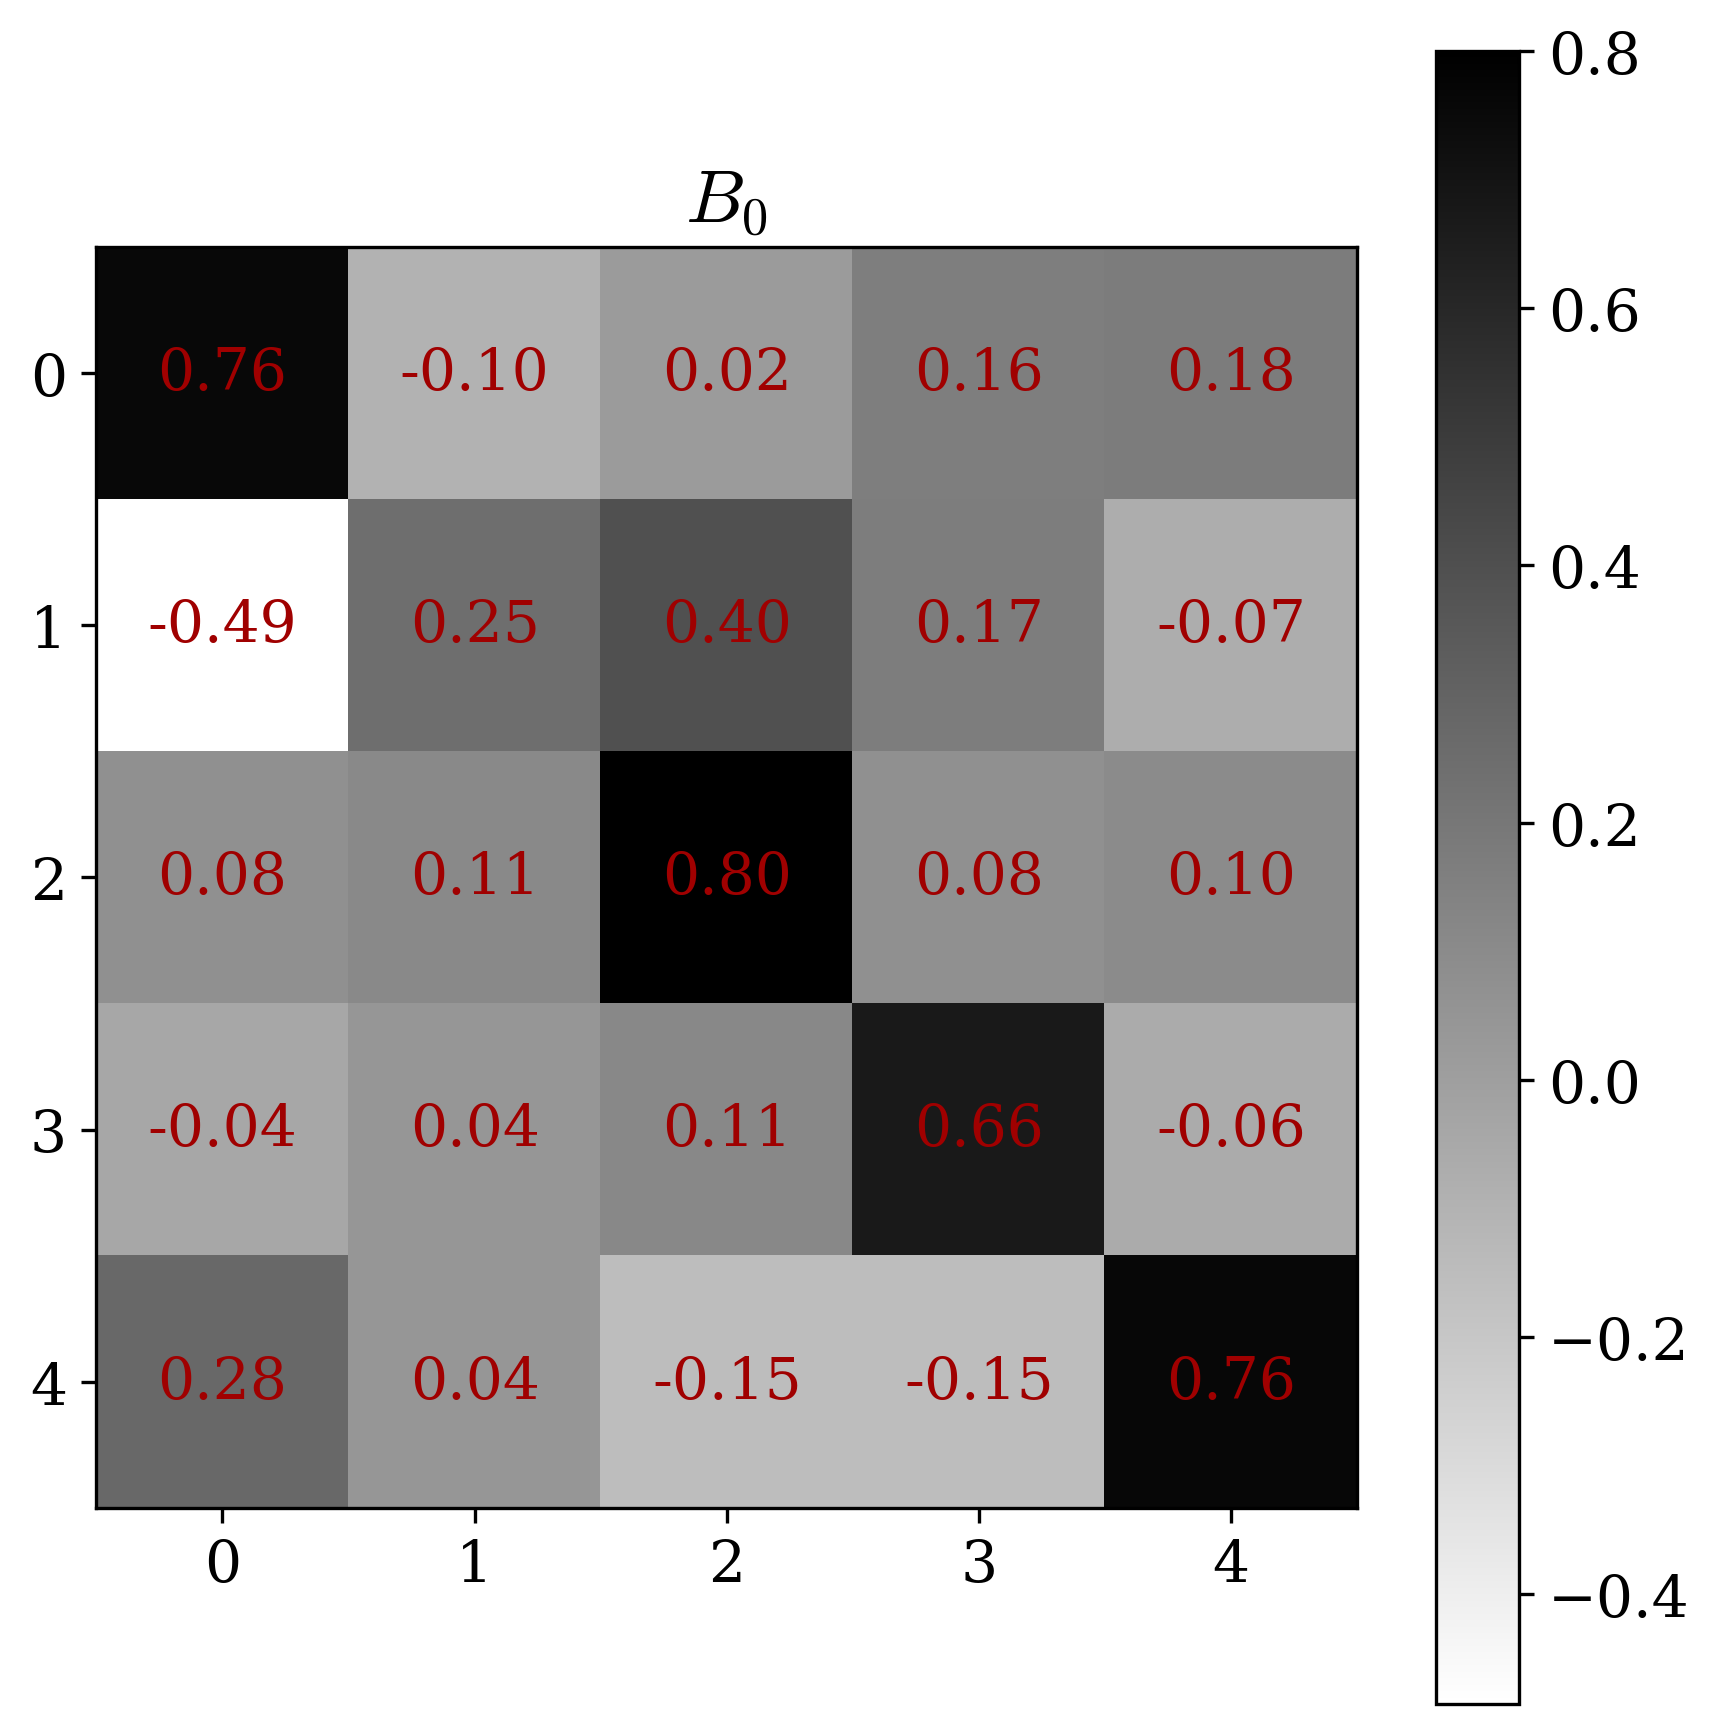
\includegraphics[width=0.72\linewidth]{cre_t4_b0_heatmap.png}
  \caption{CRE final heatmap for $B_0$ in the relaxed setting.}
  \label{fig:cre_t4_heatmap}
\end{figure}

\section{Extension Study: Context Length}
The context-length experiment introduces a sample-complexity viewpoint. With more examples in the prompt, each method receives more information about the task. Figure \ref{fig:variable_n} compares a three-layer linear Transformer, three-step GD, three-step preconditioned GD, and OLS across context lengths.

\begin{figure}[!t]
  \centering
  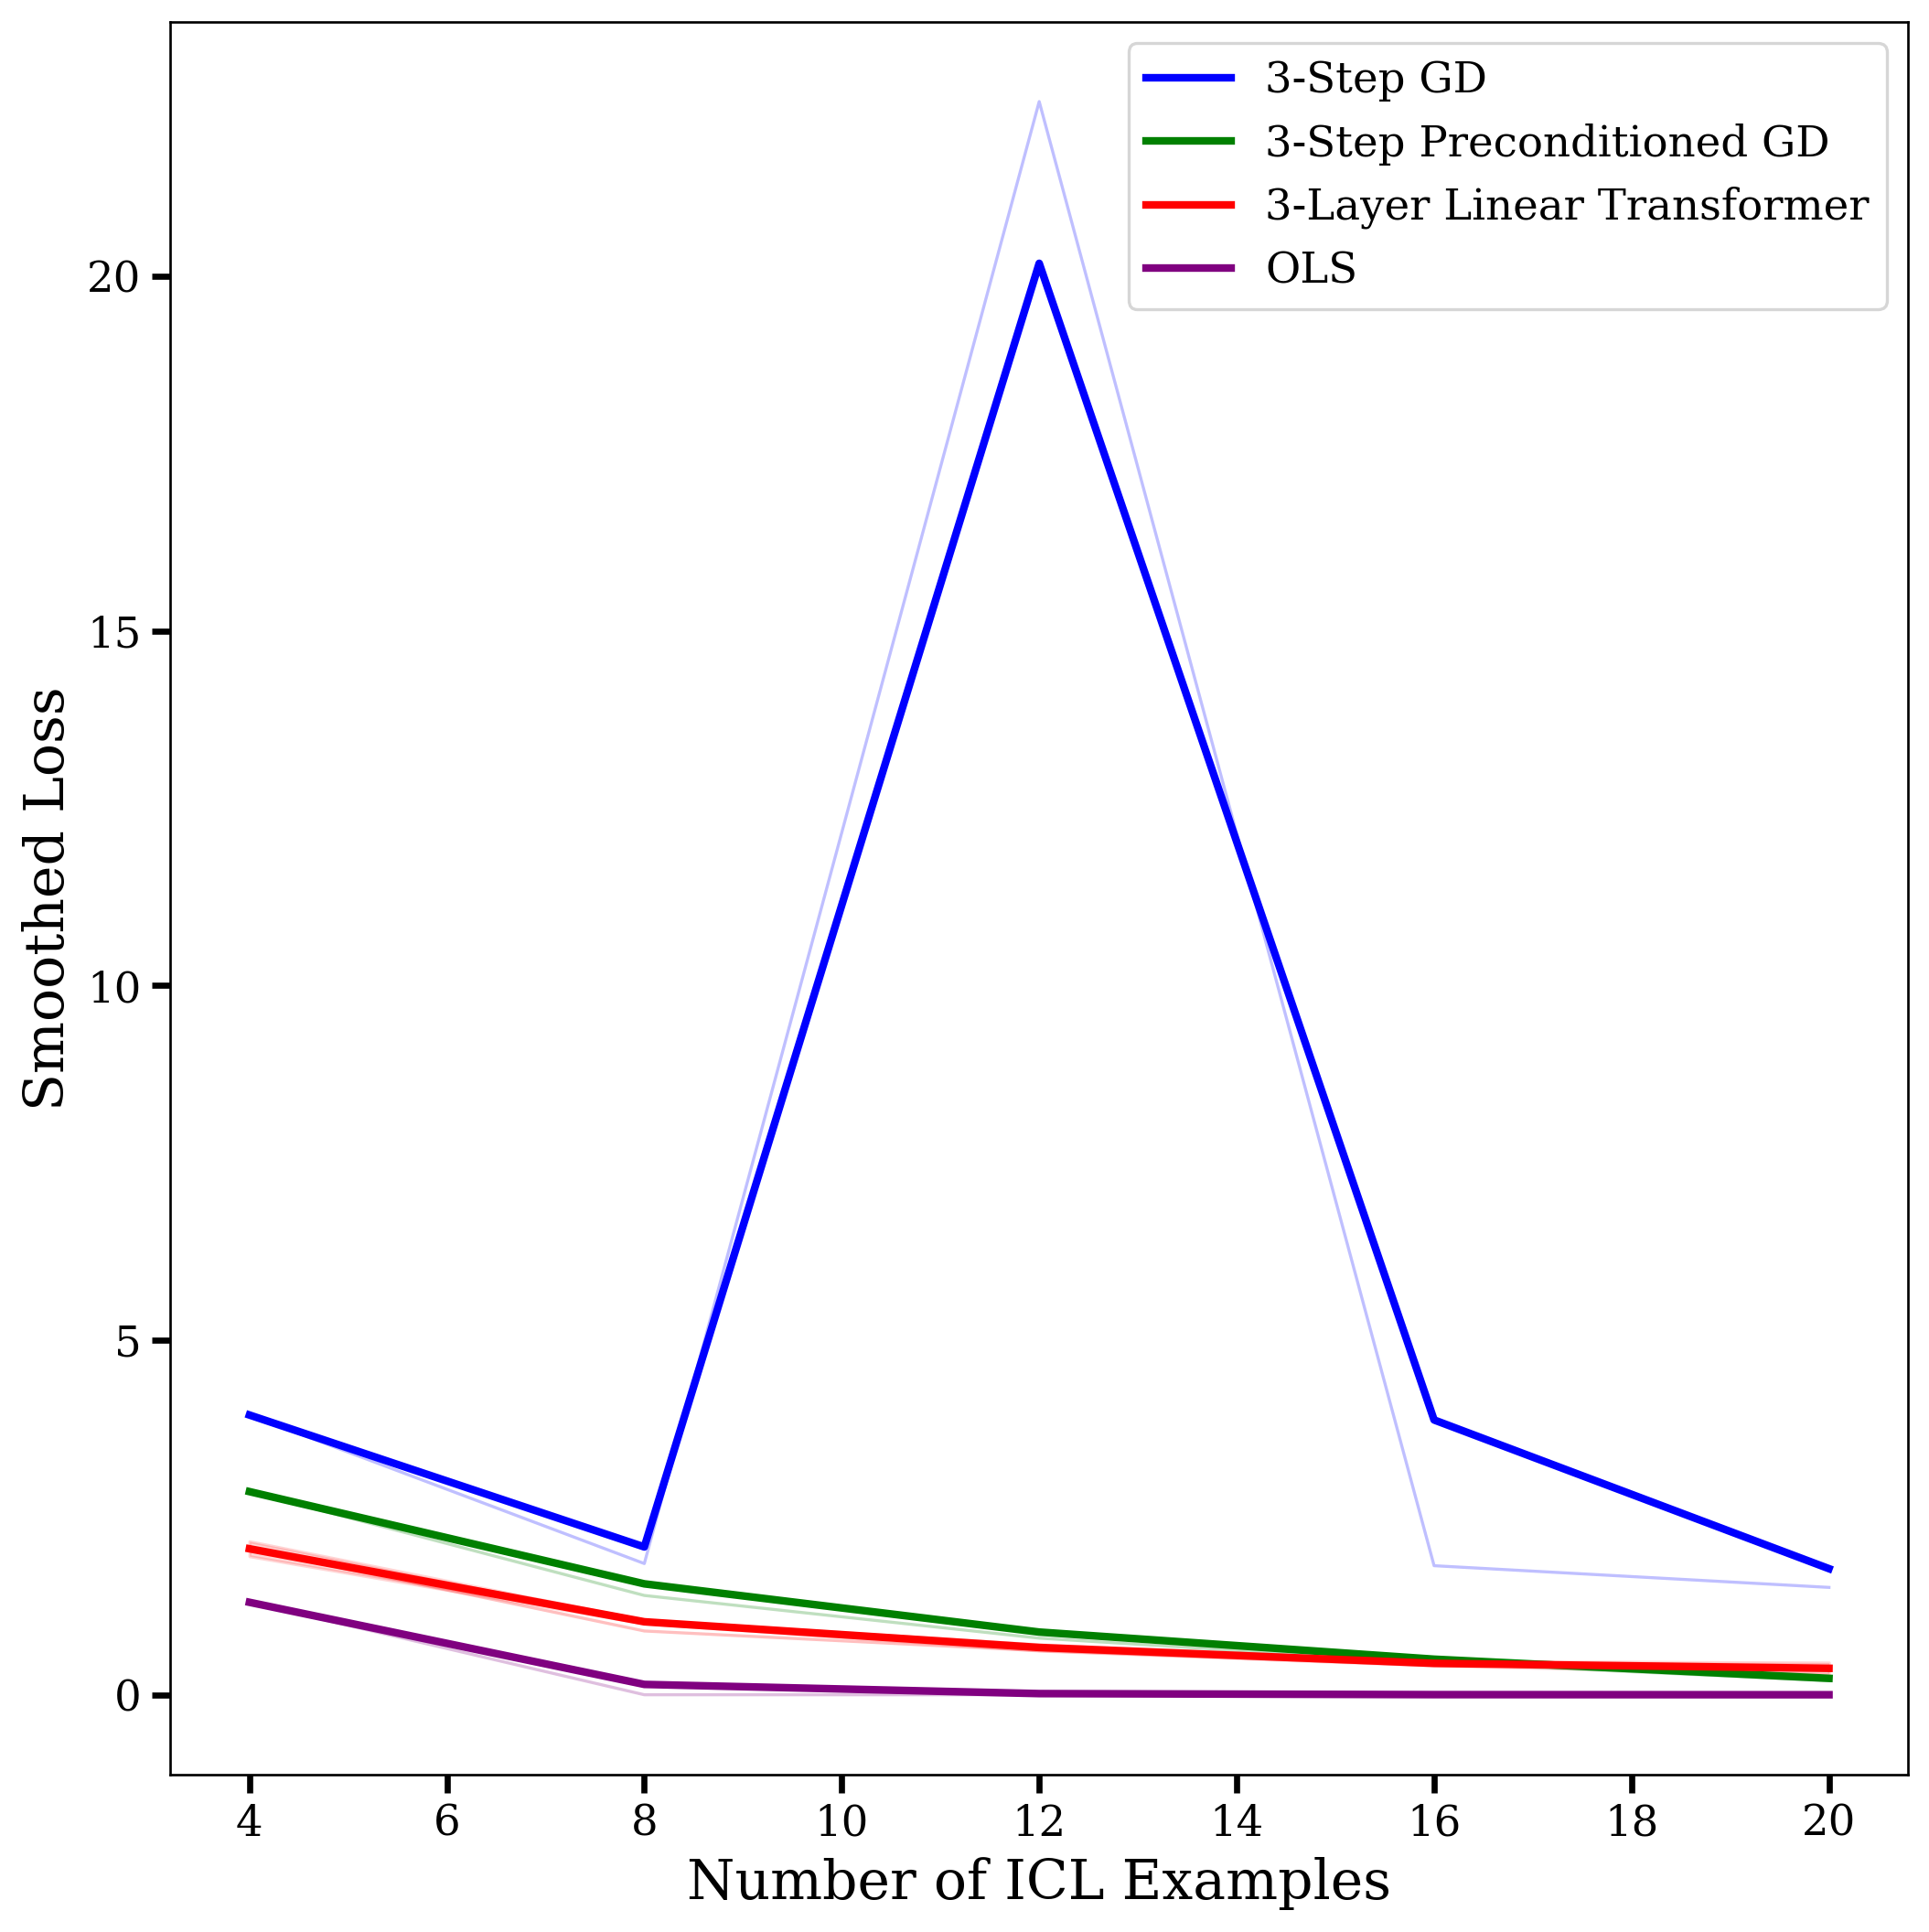
\includegraphics[width=\linewidth]{cre_variable_n_smooth.png}
  \caption{CRE context-length extension. Test loss generally improves as the number of in-context examples increases.}
  \label{fig:variable_n}
\end{figure}

\begin{table}[!t]
\centering
\caption{CRE context-length summary. Values are mean test losses.}
\label{tab:variable_n}
\begin{tabular}{rrrrr}
\toprule
$N$ & Transformer & GD & PGD & OLS\\
\midrule
4 & 2.0586 & 3.9445 & 2.8644 & 1.3038\\
8 & 0.8993 & 1.8499 & 1.4001 & 0.0000\\
12 & 0.6211 & 22.4652 & 0.7983 & 0.0000\\
16 & 0.4147 & 1.8198 & 0.4534 & 0.0000\\
20 & 0.3640 & 1.5138 & 0.1976 & 0.0000\\
\bottomrule
\end{tabular}
\end{table}

The Transformer loss decreases from $2.058553$ at $N=4$ to $0.363965$ at $N=20$. Preconditioned GD also improves strongly, from $2.864391$ to $0.197570$. OLS becomes nearly exact once enough examples are available. The visible spike at $N=12$ is a GD-specific anomaly rather than the main Transformer trend. It is best interpreted as a finite-step optimization sensitivity: with only three GD steps, a grid-searched fixed stepsize, and a non-isotropic covariance structure, the unpreconditioned update can overshoot or amplify poorly conditioned directions for a particular context length. The absence of a comparable spike in PGD supports the paper's broader message that covariance-aware preconditioning stabilizes optimization. This extension reinforces the main message: preconditioning matters for optimization, while more context reduces the statistical uncertainty of the task.

The comparison also clarifies the role of the Transformer. The trained linear Transformer is not always the best possible estimator; OLS is a strong closed-form reference when enough samples are available. The value of the Transformer result is mechanistic: it shows that a trained attention model can approximate an iterative optimizer from prompt data. The variable-$N$ experiment therefore complements, rather than replaces, the structural Theorem 3 and Theorem 4 experiments.

\subsection{Bias-Variance and Algorithmic Efficiency}
The context-length experiment can be read through a bias-variance lens. With very few examples, every method suffers from uncertainty about $\wstar$. OLS has low bias but can be unstable when information is scarce or the system is underdetermined. Gradient-based methods introduce an algorithmic bias through the number of steps and step-size choice. Preconditioned GD changes this bias by adapting the update geometry to the covariance. A trained Transformer inherits a similar algorithmic constraint: with a fixed number of layers, it can only perform a fixed number of learned updates.

This makes the finite-depth Transformer a computationally constrained estimator. Increasing $N$ improves the available statistical information, but the model still has only three learned update steps in our CRE experiment. The fact that loss decreases with $N$ means the learned iterative computation can use the additional examples, while the gap to OLS shows that finite-depth learned optimization is not the same as solving the full least-squares problem exactly.

\section{Discussion}
The paper's main contribution is to shift the explanation of ICL from expressivity alone to training-induced algorithmic structure. It is one thing to construct weights that simulate gradient descent; it is stronger to show that global optima or near-critical points of the training objective have that form. This makes the work a learning-theory paper rather than only a Transformer architecture paper.

The reproduction supports the theory at the structural level. In Theorem 3, the important observation is not merely that loss decreases, but that the covariance-adjusted matrices become closer to scaled identity than the raw matrices. In Theorem 4, the joint movement of $A_i$ and $B_i$ supports the interpretation that relaxed linear attention learns more than conventional gradient descent. The extension experiment adds a practical comparison among Transformer, GD, preconditioned GD, and OLS as context length changes.

The limitations should be stated carefully. The analysis applies to linear attention, Gaussian linear-regression tasks, and carefully defined parameter regimes. It does not prove that all large language models implement gradient descent in the same way. It also does not characterize every critical point of the non-convex training objective. From a reproduction perspective, CRE is designed to validate trends and structural consistency rather than reproduce every paper-scale numerical setting.

\subsection{Possible Extensions}
There are several natural extensions. First, the most direct theoretical extension is to analyze softmax attention. The target paper deliberately removes softmax to make the loss landscape tractable, but practical Transformers use nonlinear attention. Second, one could study richer task distributions beyond Gaussian linear regression, such as sparse linear models, nonlinear regression, or classification tasks. Third, the reproduction could be expanded by running more random seeds and larger training budgets to estimate variance in the structural metrics. Finally, the loss landscape could be studied beyond the specific critical structures identified in the paper, because non-convex objectives may contain multiple qualitatively different stationary points.

\subsection{Implications for Learning Theory}
The project illustrates a useful pattern for learning-theory analysis of modern architectures. Rather than treating a neural network as an opaque predictor, one can ask what algorithm is induced by training. If a trained model implements a known optimization method, then classical concepts such as conditioning, step size, preconditioning, and sample size become available for interpreting neural behavior. This does not solve the full theory of ICL, but it gives a concrete bridge between Transformer computation and optimization theory.

\begin{figure}[!t]
  \centering
  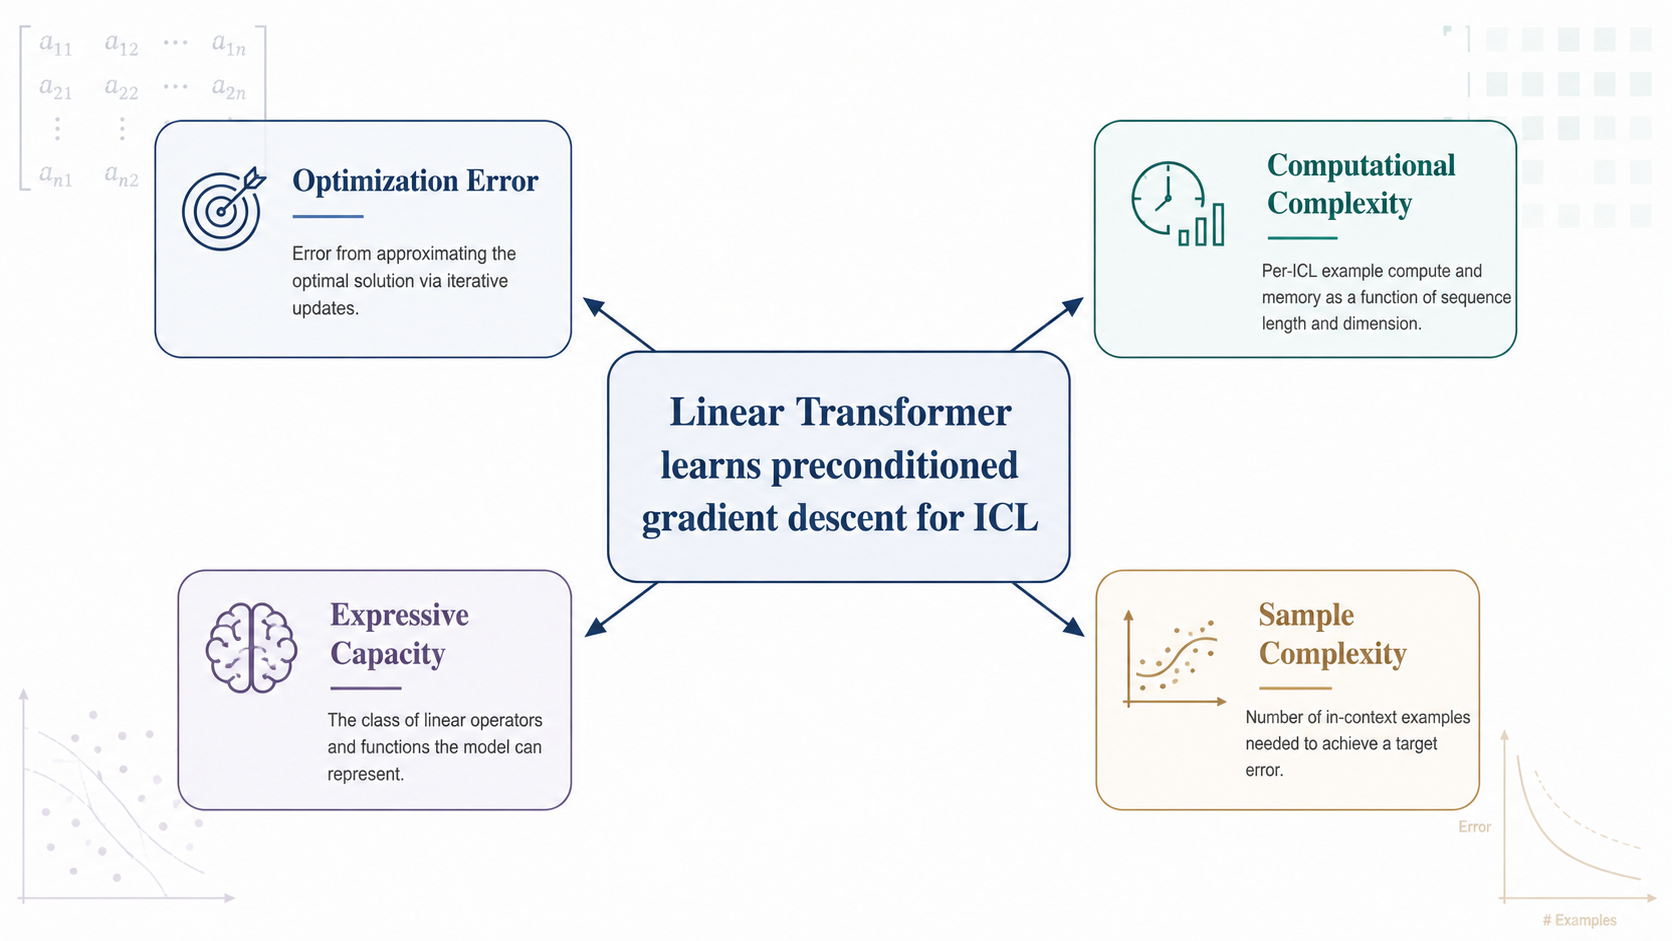
\includegraphics[width=\linewidth]{ai_summary.png}
  \caption{Summary of the course interpretation: optimization error, computational complexity, expressive capacity, and sample complexity meet in the learned-optimization view of ICL.}
  \label{fig:ai_summary}
\end{figure}

\section{Conclusion}
Ahn et al.'s NeurIPS 2023 paper provides a precise mechanism by which trained linear Transformers can implement preconditioned gradient descent for in-context learning. The central lesson is that attention layers can be interpreted as learned optimization steps, with covariance-aware preconditioning and, in the relaxed setting, feature transformations that improve conditioning. Our course-scale reproduction confirms the main qualitative signatures: decreasing ICL loss, rotated matrices approaching scaled identity structures, learned feature transformations, and improved performance with more in-context examples. The project therefore connects the course themes of optimization error, computational complexity, approximation capacity, and sample complexity within a single theoretically grounded Transformer setting.

\bibliographystyle{IEEEtran}
\bibliography{references}

\end{document}
